% Options for packages loaded elsewhere
\PassOptionsToPackage{unicode}{hyperref}
\PassOptionsToPackage{hyphens}{url}
%
\documentclass[
]{article}
\usepackage{amsmath,amssymb}
\usepackage{lmodern}
\usepackage{ifxetex,ifluatex}
\ifnum 0\ifxetex 1\fi\ifluatex 1\fi=0 % if pdftex
  \usepackage[T1]{fontenc}
  \usepackage[utf8]{inputenc}
  \usepackage{textcomp} % provide euro and other symbols
\else % if luatex or xetex
  \usepackage{unicode-math}
  \defaultfontfeatures{Scale=MatchLowercase}
  \defaultfontfeatures[\rmfamily]{Ligatures=TeX,Scale=1}
\fi
% Use upquote if available, for straight quotes in verbatim environments
\IfFileExists{upquote.sty}{\usepackage{upquote}}{}
\IfFileExists{microtype.sty}{% use microtype if available
  \usepackage[]{microtype}
  \UseMicrotypeSet[protrusion]{basicmath} % disable protrusion for tt fonts
}{}
\makeatletter
\@ifundefined{KOMAClassName}{% if non-KOMA class
  \IfFileExists{parskip.sty}{%
    \usepackage{parskip}
  }{% else
    \setlength{\parindent}{0pt}
    \setlength{\parskip}{6pt plus 2pt minus 1pt}}
}{% if KOMA class
  \KOMAoptions{parskip=half}}
\makeatother
\usepackage{xcolor}
\IfFileExists{xurl.sty}{\usepackage{xurl}}{} % add URL line breaks if available
\IfFileExists{bookmark.sty}{\usepackage{bookmark}}{\usepackage{hyperref}}
\hypersetup{
  pdftitle={Artificial Stupidity Predicting NYC AirBnB Rent},
  pdfauthor={Minghao Du},
  hidelinks,
  pdfcreator={LaTeX via pandoc}}
\urlstyle{same} % disable monospaced font for URLs
\usepackage[margin=1in]{geometry}
\usepackage{color}
\usepackage{fancyvrb}
\newcommand{\VerbBar}{|}
\newcommand{\VERB}{\Verb[commandchars=\\\{\}]}
\DefineVerbatimEnvironment{Highlighting}{Verbatim}{commandchars=\\\{\}}
% Add ',fontsize=\small' for more characters per line
\usepackage{framed}
\definecolor{shadecolor}{RGB}{248,248,248}
\newenvironment{Shaded}{\begin{snugshade}}{\end{snugshade}}
\newcommand{\AlertTok}[1]{\textcolor[rgb]{0.94,0.16,0.16}{#1}}
\newcommand{\AnnotationTok}[1]{\textcolor[rgb]{0.56,0.35,0.01}{\textbf{\textit{#1}}}}
\newcommand{\AttributeTok}[1]{\textcolor[rgb]{0.77,0.63,0.00}{#1}}
\newcommand{\BaseNTok}[1]{\textcolor[rgb]{0.00,0.00,0.81}{#1}}
\newcommand{\BuiltInTok}[1]{#1}
\newcommand{\CharTok}[1]{\textcolor[rgb]{0.31,0.60,0.02}{#1}}
\newcommand{\CommentTok}[1]{\textcolor[rgb]{0.56,0.35,0.01}{\textit{#1}}}
\newcommand{\CommentVarTok}[1]{\textcolor[rgb]{0.56,0.35,0.01}{\textbf{\textit{#1}}}}
\newcommand{\ConstantTok}[1]{\textcolor[rgb]{0.00,0.00,0.00}{#1}}
\newcommand{\ControlFlowTok}[1]{\textcolor[rgb]{0.13,0.29,0.53}{\textbf{#1}}}
\newcommand{\DataTypeTok}[1]{\textcolor[rgb]{0.13,0.29,0.53}{#1}}
\newcommand{\DecValTok}[1]{\textcolor[rgb]{0.00,0.00,0.81}{#1}}
\newcommand{\DocumentationTok}[1]{\textcolor[rgb]{0.56,0.35,0.01}{\textbf{\textit{#1}}}}
\newcommand{\ErrorTok}[1]{\textcolor[rgb]{0.64,0.00,0.00}{\textbf{#1}}}
\newcommand{\ExtensionTok}[1]{#1}
\newcommand{\FloatTok}[1]{\textcolor[rgb]{0.00,0.00,0.81}{#1}}
\newcommand{\FunctionTok}[1]{\textcolor[rgb]{0.00,0.00,0.00}{#1}}
\newcommand{\ImportTok}[1]{#1}
\newcommand{\InformationTok}[1]{\textcolor[rgb]{0.56,0.35,0.01}{\textbf{\textit{#1}}}}
\newcommand{\KeywordTok}[1]{\textcolor[rgb]{0.13,0.29,0.53}{\textbf{#1}}}
\newcommand{\NormalTok}[1]{#1}
\newcommand{\OperatorTok}[1]{\textcolor[rgb]{0.81,0.36,0.00}{\textbf{#1}}}
\newcommand{\OtherTok}[1]{\textcolor[rgb]{0.56,0.35,0.01}{#1}}
\newcommand{\PreprocessorTok}[1]{\textcolor[rgb]{0.56,0.35,0.01}{\textit{#1}}}
\newcommand{\RegionMarkerTok}[1]{#1}
\newcommand{\SpecialCharTok}[1]{\textcolor[rgb]{0.00,0.00,0.00}{#1}}
\newcommand{\SpecialStringTok}[1]{\textcolor[rgb]{0.31,0.60,0.02}{#1}}
\newcommand{\StringTok}[1]{\textcolor[rgb]{0.31,0.60,0.02}{#1}}
\newcommand{\VariableTok}[1]{\textcolor[rgb]{0.00,0.00,0.00}{#1}}
\newcommand{\VerbatimStringTok}[1]{\textcolor[rgb]{0.31,0.60,0.02}{#1}}
\newcommand{\WarningTok}[1]{\textcolor[rgb]{0.56,0.35,0.01}{\textbf{\textit{#1}}}}
\usepackage{graphicx}
\makeatletter
\def\maxwidth{\ifdim\Gin@nat@width>\linewidth\linewidth\else\Gin@nat@width\fi}
\def\maxheight{\ifdim\Gin@nat@height>\textheight\textheight\else\Gin@nat@height\fi}
\makeatother
% Scale images if necessary, so that they will not overflow the page
% margins by default, and it is still possible to overwrite the defaults
% using explicit options in \includegraphics[width, height, ...]{}
\setkeys{Gin}{width=\maxwidth,height=\maxheight,keepaspectratio}
% Set default figure placement to htbp
\makeatletter
\def\fps@figure{htbp}
\makeatother
\setlength{\emergencystretch}{3em} % prevent overfull lines
\providecommand{\tightlist}{%
  \setlength{\itemsep}{0pt}\setlength{\parskip}{0pt}}
\setcounter{secnumdepth}{-\maxdimen} % remove section numbering
\ifluatex
  \usepackage{selnolig}  % disable illegal ligatures
\fi

\title{Artificial Stupidity Predicting NYC AirBnB Rent}
\author{Minghao Du}
\date{2021-12-04}

\begin{document}
\maketitle

\hypertarget{intro}{%
\subsection{Intro}\label{intro}}

The objective of this project is to predict Airbnb rent based on 90
features. These features include various data types, and data cleaning
and pre-processing is required before modeling. The result will be
evaluated with RMSE, the lower the score is the better the model
predicts.

\hypertarget{initiating-r-environment}{%
\subsection{Initiating R Environment}\label{initiating-r-environment}}

The following code will initiate the R environment with required R
packages and helper functions. Since the project will create an
artificial neural network, TensorFlow and Keras is imported with
miniconda, of which will facilitate any GPU computation that is needed
for the network. Other than that, the flowing code also sets constant
value for the entire project, including seed and number of cores.

\begin{verbatim}
##          used (Mb) gc trigger (Mb) max used (Mb)
## Ncells 417051 22.3     872104 46.6   638940 34.2
## Vcells 769100  5.9    8388608 64.0  1635956 12.5
\end{verbatim}

\begin{verbatim}
## Command for sourcing the URL:
##   downloader::source_url("https://raw.githubusercontent.com/DMinghao/Analysis_Pocketknife/main/R/init_env.R", sha="9e657bc82974025a094b66de35cb78eb826621ab")
\end{verbatim}

\begin{verbatim}
## Hash 9e657bc82974025a094b66de35cb78eb826621ab matches expected value.
\end{verbatim}

\begin{verbatim}
## Loading required package: ggplot2
\end{verbatim}

\begin{verbatim}
## 
## Attaching package: 'plotly'
\end{verbatim}

\begin{verbatim}
## The following object is masked from 'package:ggplot2':
## 
##     last_plot
\end{verbatim}

\begin{verbatim}
## The following object is masked from 'package:stats':
## 
##     filter
\end{verbatim}

\begin{verbatim}
## The following object is masked from 'package:graphics':
## 
##     layout
\end{verbatim}

\begin{verbatim}
## -- Attaching packages --------------------------------------- tidyverse 1.3.1 --
\end{verbatim}

\begin{verbatim}
## v tibble  3.1.1     v dplyr   1.0.6
## v tidyr   1.1.3     v stringr 1.4.0
## v readr   1.4.0     v forcats 0.5.1
## v purrr   0.3.4
\end{verbatim}

\begin{verbatim}
## -- Conflicts ------------------------------------------ tidyverse_conflicts() --
## x dplyr::filter() masks plotly::filter(), stats::filter()
## x dplyr::lag()    masks stats::lag()
\end{verbatim}

\begin{verbatim}
## Registered S3 method overwritten by 'GGally':
##   method from   
##   +.gg   ggplot2
\end{verbatim}

\begin{verbatim}
## 
## Attaching package: 'psych'
\end{verbatim}

\begin{verbatim}
## The following objects are masked from 'package:ggplot2':
## 
##     %+%, alpha
\end{verbatim}

\begin{verbatim}
## 
## Attaching package: 'janitor'
\end{verbatim}

\begin{verbatim}
## The following objects are masked from 'package:stats':
## 
##     chisq.test, fisher.test
\end{verbatim}

\begin{verbatim}
## 
## Attaching package: 'lubridate'
\end{verbatim}

\begin{verbatim}
## The following objects are masked from 'package:base':
## 
##     date, intersect, setdiff, union
\end{verbatim}

\begin{verbatim}
## 
## Attaching package: 'xgboost'
\end{verbatim}

\begin{verbatim}
## The following object is masked from 'package:dplyr':
## 
##     slice
\end{verbatim}

\begin{verbatim}
## The following object is masked from 'package:plotly':
## 
##     slice
\end{verbatim}

\begin{verbatim}
## Loading required package: lattice
\end{verbatim}

\begin{verbatim}
## 
## Attaching package: 'caret'
\end{verbatim}

\begin{verbatim}
## The following object is masked from 'package:tensorflow':
## 
##     train
\end{verbatim}

\begin{verbatim}
## The following object is masked from 'package:purrr':
## 
##     lift
\end{verbatim}

\begin{verbatim}
## Loading required package: koRpus.lang.en
\end{verbatim}

\begin{verbatim}
## Loading required package: koRpus
\end{verbatim}

\begin{verbatim}
## Loading required package: sylly
\end{verbatim}

\begin{verbatim}
## 
## Attaching package: 'sylly'
\end{verbatim}

\begin{verbatim}
## The following object is masked from 'package:psych':
## 
##     describe
\end{verbatim}

\begin{verbatim}
## For information on available language packages for 'koRpus', run
## 
##   available.koRpus.lang()
## 
## and see ?install.koRpus.lang()
\end{verbatim}

\begin{verbatim}
## 
## Attaching package: 'koRpus'
\end{verbatim}

\begin{verbatim}
## The following object is masked from 'package:readr':
## 
##     tokenize
\end{verbatim}

\begin{verbatim}
## Loading required package: NLP
\end{verbatim}

\begin{verbatim}
## 
## Attaching package: 'NLP'
\end{verbatim}

\begin{verbatim}
## The following object is masked from 'package:ggplot2':
## 
##     annotate
\end{verbatim}

\begin{verbatim}
## 
## Attaching package: 'tm'
\end{verbatim}

\begin{verbatim}
## The following object is masked from 'package:koRpus':
## 
##     readTagged
\end{verbatim}

\begin{verbatim}
## Loading required package: ParamHelpers
\end{verbatim}

\begin{verbatim}
## Loading required package: checkmate
\end{verbatim}

\begin{verbatim}
## Loading required package: mlr
\end{verbatim}

\begin{verbatim}
## Warning message: 'mlr' is in 'maintenance-only' mode since July 2019.
## Future development will only happen in 'mlr3'
## (<https://mlr3.mlr-org.com>). Due to the focus on 'mlr3' there might be
## uncaught bugs meanwhile in {mlr} - please consider switching.
\end{verbatim}

\begin{verbatim}
## 
## Attaching package: 'mlr'
\end{verbatim}

\begin{verbatim}
## The following object is masked from 'package:caret':
## 
##     train
\end{verbatim}

\begin{verbatim}
## The following object is masked from 'package:tensorflow':
## 
##     train
\end{verbatim}

\begin{verbatim}
## The following object is masked from 'package:e1071':
## 
##     impute
\end{verbatim}

\begin{verbatim}
## 
## Attaching package: 'DiceKriging'
\end{verbatim}

\begin{verbatim}
## The following object is masked from 'package:checkmate':
## 
##     checkNames
\end{verbatim}

\begin{verbatim}
## 
## Attaching package: 'mice'
\end{verbatim}

\begin{verbatim}
## The following object is masked from 'package:stats':
## 
##     filter
\end{verbatim}

\begin{verbatim}
## The following objects are masked from 'package:base':
## 
##     cbind, rbind
\end{verbatim}

\begin{verbatim}
## 
## Attaching package: 'dbscan'
\end{verbatim}

\begin{verbatim}
## The following object is masked from 'package:fpc':
## 
##     dbscan
\end{verbatim}

\begin{verbatim}
## 
## Attaching package: 'reshape2'
\end{verbatim}

\begin{verbatim}
## The following object is masked from 'package:tidyr':
## 
##     smiths
\end{verbatim}

\begin{verbatim}
## [1] "Miniconda is already installed. "
## [1] "r_tf_gpu  is already installed. "
\end{verbatim}

\hypertarget{read-provided-data}{%
\subsection{Read Provided Data}\label{read-provided-data}}

The provided data is broken down to two separate files, one for
training, of which contain a price column, and a scoring data set that
does not have the price column.

\begin{Shaded}
\begin{Highlighting}[]
\NormalTok{writeSubmit }\OtherTok{\textless{}{-}} \ControlFlowTok{function}\NormalTok{(pred) \{}
\NormalTok{  submissionFile }\OtherTok{=} \FunctionTok{data.frame}\NormalTok{(}\AttributeTok{id =}\NormalTok{ scoringData}\SpecialCharTok{$}\NormalTok{id, }\AttributeTok{price =}\NormalTok{ pred)}
  \FunctionTok{write.csv}\NormalTok{(submissionFile, }\StringTok{\textquotesingle{}submission.csv\textquotesingle{}}\NormalTok{, }\AttributeTok{row.names =}\NormalTok{ F)}
\NormalTok{\}}

\NormalTok{rawData }\OtherTok{\textless{}{-}} \FunctionTok{read\_csv}\NormalTok{(}\StringTok{\textquotesingle{}./input/rentlala2021/analysisData.csv\textquotesingle{}}\NormalTok{)}
\end{Highlighting}
\end{Shaded}

\begin{verbatim}
## 
## -- Column specification --------------------------------------------------------
## cols(
##   .default = col_double(),
##   name = col_character(),
##   summary = col_character(),
##   space = col_character(),
##   description = col_character(),
##   neighborhood_overview = col_character(),
##   notes = col_character(),
##   transit = col_character(),
##   access = col_character(),
##   interaction = col_character(),
##   house_rules = col_character(),
##   host_name = col_character(),
##   host_since = col_date(format = ""),
##   host_location = col_character(),
##   host_about = col_character(),
##   host_response_time = col_character(),
##   host_response_rate = col_character(),
##   host_acceptance_rate = col_character(),
##   host_is_superhost = col_logical(),
##   host_neighbourhood = col_character(),
##   host_verifications = col_character()
##   # ... with 29 more columns
## )
## i Use `spec()` for the full column specifications.
\end{verbatim}

\begin{Shaded}
\begin{Highlighting}[]
\NormalTok{scoringData }\OtherTok{\textless{}{-}} \FunctionTok{read\_csv}\NormalTok{(}\StringTok{\textquotesingle{}./input/rentlala2021/scoringData.csv\textquotesingle{}}\NormalTok{)}
\end{Highlighting}
\end{Shaded}

\begin{verbatim}
## 
## -- Column specification --------------------------------------------------------
## cols(
##   .default = col_double(),
##   name = col_character(),
##   summary = col_character(),
##   space = col_character(),
##   description = col_character(),
##   neighborhood_overview = col_character(),
##   notes = col_character(),
##   transit = col_character(),
##   access = col_character(),
##   interaction = col_character(),
##   house_rules = col_character(),
##   host_name = col_character(),
##   host_since = col_date(format = ""),
##   host_location = col_character(),
##   host_about = col_character(),
##   host_response_time = col_character(),
##   host_response_rate = col_character(),
##   host_acceptance_rate = col_character(),
##   host_is_superhost = col_logical(),
##   host_neighbourhood = col_character(),
##   host_verifications = col_character()
##   # ... with 30 more columns
## )
## i Use `spec()` for the full column specifications.
\end{verbatim}

\hypertarget{correcting-column-data-type}{%
\subsubsection{Correcting column data
type}\label{correcting-column-data-type}}

By doing some column comparison, we can see that two data sets contains
columns that does not match each other. Thus, some preliminary house
keeping is needed to keep all columns in two data set in sync.

\begin{Shaded}
\begin{Highlighting}[]
\FunctionTok{compare\_df\_cols}\NormalTok{(rawData, scoringData) }\SpecialCharTok{\%\textgreater{}\%}
  \FunctionTok{filter}\NormalTok{(rawData }\SpecialCharTok{!=}\NormalTok{ scoringData }\SpecialCharTok{|}
\NormalTok{           rawData }\SpecialCharTok{\%\textgreater{}\%} \FunctionTok{is.na}\NormalTok{() }\SpecialCharTok{|}\NormalTok{ scoringData }\SpecialCharTok{\%\textgreater{}\%} \FunctionTok{is.na}\NormalTok{())}
\end{Highlighting}
\end{Shaded}

\begin{verbatim}
##   column_name rawData scoringData
## 1       price numeric        <NA>
## 2     zipcode numeric   character
\end{verbatim}

\begin{Shaded}
\begin{Highlighting}[]
\NormalTok{rawData }\SpecialCharTok{\%\textgreater{}\%} \FunctionTok{mutate}\NormalTok{(}\AttributeTok{license =}\NormalTok{ license }\SpecialCharTok{\%\textgreater{}\%} \FunctionTok{as.logical}\NormalTok{()) }\OtherTok{{-}\textgreater{}}\NormalTok{ rawData}
\NormalTok{scoringData  }\SpecialCharTok{\%\textgreater{}\%} \FunctionTok{mutate}\NormalTok{(}\AttributeTok{zipcode =}\NormalTok{ zipcode }\SpecialCharTok{\%\textgreater{}\%} \FunctionTok{as.numeric}\NormalTok{()) }\OtherTok{{-}\textgreater{}}\NormalTok{ scoringData}
\end{Highlighting}
\end{Shaded}

\begin{verbatim}
## Warning in zipcode %>% as.numeric(): NAs introduced by coercion
\end{verbatim}

\begin{Shaded}
\begin{Highlighting}[]
\FunctionTok{compare\_df\_cols}\NormalTok{(rawData, scoringData) }\SpecialCharTok{\%\textgreater{}\%}
  \FunctionTok{filter}\NormalTok{(rawData }\SpecialCharTok{!=}\NormalTok{ scoringData }\SpecialCharTok{|}\NormalTok{ rawData }\SpecialCharTok{\%\textgreater{}\%} \FunctionTok{is.na}\NormalTok{() }\SpecialCharTok{|}\NormalTok{ scoringData }\SpecialCharTok{\%\textgreater{}\%} \FunctionTok{is.na}\NormalTok{())}
\end{Highlighting}
\end{Shaded}

\begin{verbatim}
##   column_name rawData scoringData
## 1       price numeric        <NA>
\end{verbatim}

\hypertarget{merging-scoring-data-and-training-data}{%
\subsubsection{Merging scoring data and training
data}\label{merging-scoring-data-and-training-data}}

The following code will create a price column for the scoring data such
that two data sets can bind together as one data set for the upcoming
data pre-processing and cleaning.

\begin{Shaded}
\begin{Highlighting}[]
\NormalTok{pricedScoringData }\OtherTok{\textless{}{-}}\NormalTok{ scoringData }\SpecialCharTok{\%\textgreater{}\%} \FunctionTok{mutate}\NormalTok{(}\AttributeTok{price =} \SpecialCharTok{{-}}\DecValTok{1}\NormalTok{)}

\NormalTok{allData }\OtherTok{\textless{}{-}}\NormalTok{ rawData }\SpecialCharTok{\%\textgreater{}\%} \FunctionTok{bind\_rows}\NormalTok{(pricedScoringData) }
\end{Highlighting}
\end{Shaded}

\hypertarget{pre-processing-data}{%
\subsection{Pre-Processing Data}\label{pre-processing-data}}

Due to the fact that most models can not handle missing data, character
data, or unscaled data, it would be necessary to clean and preprocess
data before moving forward. Other than that, it might be helpful to do
some feature engineering such that models can have more data to work
with. However, considering the fact that most models tend to run longer
and perform worse with more feature added, feature selection will be
needed to improve model performance and/or accuracy.

\hypertarget{grouping-columns-with-same-data-type}{%
\subsubsection{Grouping Columns with Same Data
Type}\label{grouping-columns-with-same-data-type}}

Given that there are different data types in the data set, bulk
processing columns with the same data type might speed up the process.
The following code serves the purpose of putting columns with same data
type together to help with later data cleaning.

\begin{Shaded}
\begin{Highlighting}[]
\CommentTok{\# Extract ID column }
\NormalTok{extractID }\OtherTok{\textless{}{-}}\NormalTok{ allData }\SpecialCharTok{\%\textgreater{}\%} \FunctionTok{select}\NormalTok{(id)}

\NormalTok{allData }\OtherTok{\textless{}{-}}\NormalTok{ allData }\SpecialCharTok{\%\textgreater{}\%} \FunctionTok{select}\NormalTok{(}\SpecialCharTok{{-}}\NormalTok{id)}

\CommentTok{\# Put similar columns into baskets }
\NormalTok{numericCols }\OtherTok{\textless{}{-}}\NormalTok{ allData }\SpecialCharTok{\%\textgreater{}\%} \FunctionTok{select}\NormalTok{(is.numeric) }\SpecialCharTok{\%\textgreater{}\%} \FunctionTok{colnames}\NormalTok{()}
\NormalTok{boolCols }\OtherTok{\textless{}{-}}\NormalTok{ allData }\SpecialCharTok{\%\textgreater{}\%} \FunctionTok{select}\NormalTok{(is.logical) }\SpecialCharTok{\%\textgreater{}\%} \FunctionTok{colnames}\NormalTok{()}
\NormalTok{dateCols }\OtherTok{\textless{}{-}}\NormalTok{ allData }\SpecialCharTok{\%\textgreater{}\%} \FunctionTok{select}\NormalTok{(is.Date) }\SpecialCharTok{\%\textgreater{}\%} \FunctionTok{colnames}\NormalTok{()}
\NormalTok{charCols }\OtherTok{\textless{}{-}}\NormalTok{ allData }\SpecialCharTok{\%\textgreater{}\%} \FunctionTok{select}\NormalTok{(is.character) }\SpecialCharTok{\%\textgreater{}\%} \FunctionTok{colnames}\NormalTok{()}
\NormalTok{longCharCols }\OtherTok{\textless{}{-}}
\NormalTok{  allData[charCols] }\SpecialCharTok{\%\textgreater{}\%} 
  \FunctionTok{select}\NormalTok{(}\FunctionTok{c}\NormalTok{(name, }
\NormalTok{      summary, }
\NormalTok{      space, }
\NormalTok{      description, }
\NormalTok{      neighborhood\_overview, }
\NormalTok{      notes, }
\NormalTok{      transit, }
\NormalTok{      access, }
\NormalTok{      interaction, }
\NormalTok{      house\_rules, }
\NormalTok{      host\_about}
\NormalTok{  )) }\SpecialCharTok{\%\textgreater{}\%} 
  \FunctionTok{colnames}\NormalTok{()}
\NormalTok{factorCharCols }\OtherTok{\textless{}{-}} 
\NormalTok{  allData[charCols] }\SpecialCharTok{\%\textgreater{}\%} 
  \FunctionTok{select}\NormalTok{(}\SpecialCharTok{{-}}\FunctionTok{c}\NormalTok{(name, }
\NormalTok{      summary, }
\NormalTok{      space, }
\NormalTok{      description, }
\NormalTok{      neighborhood\_overview, }
\NormalTok{      notes, }
\NormalTok{      transit, }
\NormalTok{      access, }
\NormalTok{      interaction, }
\NormalTok{      house\_rules, }
\NormalTok{      host\_about}
\NormalTok{  )) }\SpecialCharTok{\%\textgreater{}\%} 
  \FunctionTok{select}\NormalTok{(}\SpecialCharTok{{-}}\FunctionTok{c}\NormalTok{(}
\NormalTok{    host\_name, }
\NormalTok{    host\_verifications, }
\NormalTok{    host\_response\_time,}
\NormalTok{    calendar\_updated, }
\NormalTok{    host\_response\_rate, }
\NormalTok{    host\_acceptance\_rate, }
\NormalTok{    amenities}
\NormalTok{  )) }\SpecialCharTok{\%\textgreater{}\%} 
  \FunctionTok{colnames}\NormalTok{()}

\NormalTok{rateCols }\OtherTok{\textless{}{-}}\NormalTok{ allData }\SpecialCharTok{\%\textgreater{}\%} 
  \FunctionTok{select}\NormalTok{(}\FunctionTok{c}\NormalTok{(host\_response\_rate, host\_acceptance\_rate)) }\SpecialCharTok{\%\textgreater{}\%} 
  \FunctionTok{colnames}\NormalTok{()}

\CommentTok{\# Encode all text columns to UTF{-}8 }
\NormalTok{allData[charCols] }\OtherTok{\textless{}{-}}\NormalTok{ allData[charCols] }\SpecialCharTok{\%\textgreater{}\%} \FunctionTok{mutate\_all}\NormalTok{(}\FunctionTok{funs}\NormalTok{(}\FunctionTok{enc2utf8}\NormalTok{(.)))}
\end{Highlighting}
\end{Shaded}

\hypertarget{data-wrangling-and-cleaning}{%
\subsubsection{Data Wrangling and
Cleaning}\label{data-wrangling-and-cleaning}}

Having the data in various format and type prevents us to extract
information from the data. Hence, the following section will help
transform some columns such that they will be easier to work with.

\hypertarget{zip-code-column}{%
\paragraph{Zip code column}\label{zip-code-column}}

Given that there exists some missing zip codes in the data set, we can
fill in those data point with the most common zip code in their
corresponding area.

\begin{Shaded}
\begin{Highlighting}[]
\NormalTok{mostCommonZip }\OtherTok{\textless{}{-}}\NormalTok{ allData }\SpecialCharTok{\%\textgreater{}\%} 
  \FunctionTok{select}\NormalTok{(}\FunctionTok{c}\NormalTok{(neighbourhood\_cleansed, neighbourhood\_group\_cleansed, city, zipcode)) }\SpecialCharTok{\%\textgreater{}\%} 
  \FunctionTok{group\_by}\NormalTok{(neighbourhood\_cleansed, zipcode) }\SpecialCharTok{\%\textgreater{}\%} 
  \FunctionTok{summarise}\NormalTok{(}\AttributeTok{count =} \FunctionTok{n}\NormalTok{()) }\SpecialCharTok{\%\textgreater{}\%} 
  \FunctionTok{filter}\NormalTok{(count }\SpecialCharTok{==} \FunctionTok{max}\NormalTok{(count)) }\SpecialCharTok{\%\textgreater{}\%} 
  \FunctionTok{ungroup}\NormalTok{()}
\end{Highlighting}
\end{Shaded}

\begin{verbatim}
## `summarise()` has grouped output by 'neighbourhood_cleansed'. You can override using the `.groups` argument.
\end{verbatim}

\begin{Shaded}
\begin{Highlighting}[]
\NormalTok{getZip }\OtherTok{\textless{}{-}} \ControlFlowTok{function}\NormalTok{(neighbourhood\_cleansed)\{}
\NormalTok{  mostCommonZip }\SpecialCharTok{\%\textgreater{}\%} \FunctionTok{filter}\NormalTok{(neighbourhood\_cleansed }\SpecialCharTok{==}\NormalTok{ neighbourhood\_cleansed) }\SpecialCharTok{\%\textgreater{}\%} \FunctionTok{select}\NormalTok{(zipcode) }\SpecialCharTok{\%\textgreater{}\%} \FunctionTok{pull}\NormalTok{(zipcode)}
\NormalTok{\}}

\NormalTok{allData }\OtherTok{\textless{}{-}}\NormalTok{ allData }\SpecialCharTok{\%\textgreater{}\%} \FunctionTok{mutate}\NormalTok{(}\AttributeTok{zipcode =} \FunctionTok{ifelse}\NormalTok{(}\FunctionTok{is.na}\NormalTok{(zipcode), }\FunctionTok{getZip}\NormalTok{(neighbourhood\_cleansed), zipcode)) }\SpecialCharTok{\%\textgreater{}\%} \FunctionTok{mutate}\NormalTok{(}\AttributeTok{zipcode =}\NormalTok{ zipcode }\SpecialCharTok{\%\textgreater{}\%} \FunctionTok{as.factor}\NormalTok{())}
\end{Highlighting}
\end{Shaded}

\hypertarget{rate-columns}{%
\paragraph{Rate columns}\label{rate-columns}}

There exists some text columns that are in the percentage format. We can
assume that all NA values in these columns are 0, since, in a real world
scenario, it's reasonable that theses NA values are derived from
dividing 0. For the rest of the data point, we can parse to numeric.

\begin{Shaded}
\begin{Highlighting}[]
\NormalTok{allData[rateCols] }\OtherTok{\textless{}{-}}\NormalTok{ allData[rateCols] }\SpecialCharTok{\%\textgreater{}\%} 
  \FunctionTok{mutate}\NormalTok{(}\AttributeTok{host\_response\_rate =} \FunctionTok{gsub}\NormalTok{(}\StringTok{"N/A"}\NormalTok{,}\StringTok{"0\%"}\NormalTok{, host\_response\_rate)) }\SpecialCharTok{\%\textgreater{}\%} 
  \FunctionTok{mutate}\NormalTok{(}\AttributeTok{host\_acceptance\_rate =} \FunctionTok{gsub}\NormalTok{(}\StringTok{"N/A"}\NormalTok{,}\StringTok{"0\%"}\NormalTok{, host\_acceptance\_rate)) }\SpecialCharTok{\%\textgreater{}\%} 
  \FunctionTok{mutate}\NormalTok{(}\AttributeTok{host\_response\_rate =} \FunctionTok{gsub}\NormalTok{(}\StringTok{"\%"}\NormalTok{,}\StringTok{""}\NormalTok{, host\_response\_rate)) }\SpecialCharTok{\%\textgreater{}\%} 
  \FunctionTok{mutate}\NormalTok{(}\AttributeTok{host\_acceptance\_rate =} \FunctionTok{gsub}\NormalTok{(}\StringTok{"\%"}\NormalTok{,}\StringTok{""}\NormalTok{, host\_acceptance\_rate)) }\SpecialCharTok{\%\textgreater{}\%} 
  \FunctionTok{mutate\_all}\NormalTok{(as.numeric) }\SpecialCharTok{\%\textgreater{}\%} 
  \FunctionTok{mutate\_each}\NormalTok{(}\FunctionTok{funs}\NormalTok{(.}\SpecialCharTok{/}\DecValTok{100}\NormalTok{)) }\SpecialCharTok{\%\textgreater{}\%} 
  \FunctionTok{replace}\NormalTok{(}\FunctionTok{is.na}\NormalTok{(.),}\DecValTok{0}\NormalTok{)}
\end{Highlighting}
\end{Shaded}

\begin{verbatim}
## Warning: `mutate_each_()` was deprecated in dplyr 0.7.0.
## Please use `across()` instead.
\end{verbatim}

\hypertarget{handle-non-char-columns-na-value}{%
\paragraph{Handle non-char columns NA
value}\label{handle-non-char-columns-na-value}}

The following code handles square\_feet, weekly\_price, and
monthly\_price columns' NA value. It might not be the best way, but
setting these values to 0 is safe. One alternative will be using MISE
imputation, but since the number of missing value is too large, it
tempers the distribution of these columns. Another way that can be use
is to train models that predicts these values.

\begin{Shaded}
\begin{Highlighting}[]
\NormalTok{allData[boolCols] }\OtherTok{\textless{}{-}}\NormalTok{ allData[boolCols] }\SpecialCharTok{\%\textgreater{}\%} \FunctionTok{replace}\NormalTok{(}\FunctionTok{is.na}\NormalTok{(.),F)}

\NormalTok{reservedNumCols }\OtherTok{\textless{}{-}}\NormalTok{ allData }\SpecialCharTok{\%\textgreater{}\%} \FunctionTok{select}\NormalTok{(}\FunctionTok{c}\NormalTok{(square\_feet, weekly\_price, monthly\_price)) }\SpecialCharTok{\%\textgreater{}\%} \FunctionTok{colnames}\NormalTok{()}

\NormalTok{allData[numericCols[numericCols }\SpecialCharTok{\%!in\%}\NormalTok{ reservedNumCols]] }\OtherTok{\textless{}{-}} 
\NormalTok{  allData[numericCols[numericCols }\SpecialCharTok{\%!in\%}\NormalTok{ reservedNumCols]] }\SpecialCharTok{\%\textgreater{}\%} \FunctionTok{replace}\NormalTok{(}\FunctionTok{is.na}\NormalTok{(.),}\DecValTok{0}\NormalTok{)}

\NormalTok{allData }\OtherTok{\textless{}{-}}\NormalTok{ allData }\SpecialCharTok{\%\textgreater{}\%} \FunctionTok{mutate}\NormalTok{(}\AttributeTok{square\_feet =} \FunctionTok{ifelse}\NormalTok{(}\FunctionTok{is.na}\NormalTok{(square\_feet), }\DecValTok{0}\NormalTok{, square\_feet))}
\NormalTok{allData }\OtherTok{\textless{}{-}}\NormalTok{ allData }\SpecialCharTok{\%\textgreater{}\%} \FunctionTok{mutate}\NormalTok{(}\AttributeTok{weekly\_price =} \FunctionTok{ifelse}\NormalTok{(}\FunctionTok{is.na}\NormalTok{(weekly\_price), }\DecValTok{0}\NormalTok{, weekly\_price))}
\NormalTok{allData }\OtherTok{\textless{}{-}}\NormalTok{ allData }\SpecialCharTok{\%\textgreater{}\%} \FunctionTok{mutate}\NormalTok{(}\AttributeTok{monthly\_price =} \FunctionTok{ifelse}\NormalTok{(}\FunctionTok{is.na}\NormalTok{(monthly\_price), }\DecValTok{0}\NormalTok{, monthly\_price))}
\end{Highlighting}
\end{Shaded}

\hypertarget{factor-columns}{%
\paragraph{Factor columns}\label{factor-columns}}

There exists several text columns that can be converted to factors. Some
of them are only having one level, so they should be drop. On the other
hand, I decided to keep columns with large amount of levels as well, but
it would be wise to down size these factors and grouping low frequency
factors into other.

\begin{Shaded}
\begin{Highlighting}[]
\NormalTok{allData[factorCharCols] }\OtherTok{\textless{}{-}}\NormalTok{ allData[factorCharCols] }\SpecialCharTok{\%\textgreater{}\%}
  \FunctionTok{replace}\NormalTok{(}\FunctionTok{is.na}\NormalTok{(.), }\StringTok{"N/A"}\NormalTok{) }\SpecialCharTok{\%\textgreater{}\%}
  \FunctionTok{mutate\_all}\NormalTok{(as.factor)}

\CommentTok{\# Exclude 1 level factor columns }
\NormalTok{allData }\OtherTok{\textless{}{-}}\NormalTok{ allData }\SpecialCharTok{\%\textgreater{}\%} \FunctionTok{select}\NormalTok{(}\SpecialCharTok{{-}}\FunctionTok{c}\NormalTok{(country\_code, country, state, market)) }
\end{Highlighting}
\end{Shaded}

\hypertarget{host-verification-and-amenities}{%
\paragraph{Host verification and
amenities}\label{host-verification-and-amenities}}

For host verification and amenities columns, they are being transformed
into one hot dummy columns per each unique items. This will allow models
to process information in these two columns easier. The original columns
are then dropped after being processed.

\begin{Shaded}
\begin{Highlighting}[]
\CommentTok{\# Create verification count column }
\NormalTok{allData }\OtherTok{\textless{}{-}}\NormalTok{ allData }\SpecialCharTok{\%\textgreater{}\%} 
  \FunctionTok{mutate}\NormalTok{(}\AttributeTok{host\_verifications =} \FunctionTok{gsub}\NormalTok{(}\StringTok{"}\SpecialCharTok{\textbackslash{}\textbackslash{}}\StringTok{[|}\SpecialCharTok{\textbackslash{}\textbackslash{}}\StringTok{]|}\SpecialCharTok{\textbackslash{}\textbackslash{}}\StringTok{\textquotesingle{}|}\SpecialCharTok{\textbackslash{}\textbackslash{}}\StringTok{,"}\NormalTok{, }\StringTok{""}\NormalTok{, host\_verifications)) }\SpecialCharTok{\%\textgreater{}\%} 
  \FunctionTok{mutate}\NormalTok{(}\AttributeTok{vari\_count =} \FunctionTok{strsplit}\NormalTok{(host\_verifications, }\StringTok{" "}\NormalTok{) }\SpecialCharTok{\%\textgreater{}\%} \FunctionTok{lengths}\NormalTok{())}

\NormalTok{vari\_list }\OtherTok{\textless{}{-}}\NormalTok{ allData }\SpecialCharTok{\%\textgreater{}\%} 
  \FunctionTok{select}\NormalTok{(host\_verifications) }\SpecialCharTok{\%\textgreater{}\%} 
  \FunctionTok{lapply}\NormalTok{(}\ControlFlowTok{function}\NormalTok{(x) }\FunctionTok{unique}\NormalTok{(}\FunctionTok{trimws}\NormalTok{(}\FunctionTok{unlist}\NormalTok{(}\FunctionTok{strsplit}\NormalTok{(x, }\StringTok{" "}\NormalTok{)))))}

\ControlFlowTok{for}\NormalTok{(w }\ControlFlowTok{in} \DecValTok{1}\SpecialCharTok{:}\FunctionTok{length}\NormalTok{(vari\_list[[}\DecValTok{1}\NormalTok{]])) \{}
\NormalTok{  new }\OtherTok{\textless{}{-}} \FunctionTok{grepl}\NormalTok{(}\AttributeTok{pattern =}\NormalTok{ vari\_list[[}\DecValTok{1}\NormalTok{]][w], }\AttributeTok{x =}\NormalTok{ allData}\SpecialCharTok{$}\NormalTok{host\_verifications, }\AttributeTok{fixed =} \ConstantTok{TRUE}\NormalTok{)}
\NormalTok{  allData[}\FunctionTok{paste}\NormalTok{(vari\_list[[}\DecValTok{1}\NormalTok{]][w], }\StringTok{"\_vari"}\NormalTok{)] }\OtherTok{\textless{}{-}}\NormalTok{ new}
\NormalTok{\}}

\CommentTok{\# Create amenities count column }
\NormalTok{allData }\OtherTok{\textless{}{-}}\NormalTok{ allData }\SpecialCharTok{\%\textgreater{}\%} 
  \FunctionTok{mutate}\NormalTok{(}\AttributeTok{amenities\_count =} \FunctionTok{strsplit}\NormalTok{(amenities, }\StringTok{","}\NormalTok{) }\SpecialCharTok{\%\textgreater{}\%} \FunctionTok{lengths}\NormalTok{()) }

\NormalTok{amen\_list }\OtherTok{\textless{}{-}}\NormalTok{ allData }\SpecialCharTok{\%\textgreater{}\%} 
  \FunctionTok{select}\NormalTok{(amenities) }\SpecialCharTok{\%\textgreater{}\%} 
  \FunctionTok{mutate}\NormalTok{(}\AttributeTok{amenities =} \FunctionTok{gsub}\NormalTok{(}\StringTok{"}\SpecialCharTok{\textbackslash{}\textbackslash{}}\StringTok{."}\NormalTok{, }\StringTok{""}\NormalTok{, amenities)) }\SpecialCharTok{\%\textgreater{}\%} 
  \FunctionTok{lapply}\NormalTok{(}\ControlFlowTok{function}\NormalTok{(x) }\FunctionTok{unique}\NormalTok{(}\FunctionTok{trimws}\NormalTok{(}\FunctionTok{unlist}\NormalTok{(}\FunctionTok{strsplit}\NormalTok{(x, }\StringTok{","}\NormalTok{)))))}

\ControlFlowTok{for}\NormalTok{(w }\ControlFlowTok{in} \DecValTok{1}\SpecialCharTok{:}\FunctionTok{length}\NormalTok{(amen\_list[[}\DecValTok{1}\NormalTok{]])) \{}
\NormalTok{  new }\OtherTok{\textless{}{-}} \FunctionTok{grepl}\NormalTok{(}\AttributeTok{pattern =}\NormalTok{ amen\_list[[}\DecValTok{1}\NormalTok{]][w], }\AttributeTok{x =}\NormalTok{ allData}\SpecialCharTok{$}\NormalTok{amenities, }\AttributeTok{fixed =} \ConstantTok{TRUE}\NormalTok{)}
\NormalTok{  allData[}\FunctionTok{paste}\NormalTok{(amen\_list[[}\DecValTok{1}\NormalTok{]][w], }\StringTok{"\_amen"}\NormalTok{)] }\OtherTok{\textless{}{-}}\NormalTok{ new}
\NormalTok{\}}

\CommentTok{\# discard original column }
\NormalTok{allData }\OtherTok{\textless{}{-}}\NormalTok{ allData }\SpecialCharTok{\%\textgreater{}\%} \FunctionTok{select}\NormalTok{(}\SpecialCharTok{{-}}\FunctionTok{c}\NormalTok{(amenities, host\_verifications)) }\SpecialCharTok{\%\textgreater{}\%} \FunctionTok{clean\_names}\NormalTok{()}
\end{Highlighting}
\end{Shaded}

\hypertarget{duration-columns}{%
\paragraph{Duration columns}\label{duration-columns}}

Duration columns are messy, since they are all in text format and does
not have consistent step size. Therefore after stripping all text
component in these columns, a column specific step size is chosen to
help rescaling the duration.

\begin{Shaded}
\begin{Highlighting}[]
\NormalTok{allData }\OtherTok{\textless{}{-}}\NormalTok{ allData }\SpecialCharTok{\%\textgreater{}\%}
  \FunctionTok{mutate}\NormalTok{(}\AttributeTok{host\_response\_time =} \FunctionTok{gsub}\NormalTok{(}\StringTok{"within a "}\NormalTok{, }\StringTok{""}\NormalTok{, host\_response\_time)) }\SpecialCharTok{\%\textgreater{}\%}
  \FunctionTok{mutate}\NormalTok{(}\AttributeTok{host\_response\_time =} \FunctionTok{gsub}\NormalTok{(}\StringTok{"within an "}\NormalTok{, }\StringTok{""}\NormalTok{, host\_response\_time)) }\SpecialCharTok{\%\textgreater{}\%}
  \FunctionTok{mutate}\NormalTok{(}\AttributeTok{host\_response\_time =} \FunctionTok{gsub}\NormalTok{(}\StringTok{"few hours"}\NormalTok{, }\StringTok{"12"}\NormalTok{, host\_response\_time)) }\SpecialCharTok{\%\textgreater{}\%}
  \FunctionTok{mutate}\NormalTok{(}\AttributeTok{host\_response\_time =} \FunctionTok{gsub}\NormalTok{(}\StringTok{"hour"}\NormalTok{, }\StringTok{"1"}\NormalTok{, host\_response\_time)) }\SpecialCharTok{\%\textgreater{}\%}
  \FunctionTok{mutate}\NormalTok{(}\AttributeTok{host\_response\_time =} \FunctionTok{gsub}\NormalTok{(}\StringTok{"a few days or more"}\NormalTok{, }\StringTok{"48"}\NormalTok{, host\_response\_time)) }\SpecialCharTok{\%\textgreater{}\%}
  \FunctionTok{mutate}\NormalTok{(}\AttributeTok{host\_response\_time =} \FunctionTok{gsub}\NormalTok{(}\StringTok{"day"}\NormalTok{, }\StringTok{"24"}\NormalTok{, host\_response\_time)) }\SpecialCharTok{\%\textgreater{}\%}
  \FunctionTok{mutate}\NormalTok{(}\AttributeTok{host\_response\_time =} \FunctionTok{replace\_na}\NormalTok{(host\_response\_time, }\StringTok{"N/A"}\NormalTok{)) }\SpecialCharTok{\%\textgreater{}\%} 
  \FunctionTok{mutate}\NormalTok{(}\AttributeTok{host\_response\_time =} \FunctionTok{gsub}\NormalTok{(}\StringTok{"N/A"}\NormalTok{, }\StringTok{"96"}\NormalTok{, host\_response\_time)) }\SpecialCharTok{\%\textgreater{}\%}
  \FunctionTok{mutate}\NormalTok{(}\AttributeTok{host\_response\_time =} \FunctionTok{as.numeric}\NormalTok{(host\_response\_time))}

\NormalTok{allData }\OtherTok{\textless{}{-}}\NormalTok{ allData }\SpecialCharTok{\%\textgreater{}\%} 
  \FunctionTok{mutate}\NormalTok{(}\AttributeTok{calendar\_updated =} \FunctionTok{gsub}\NormalTok{(}\StringTok{" ago"}\NormalTok{, }\StringTok{""}\NormalTok{, calendar\_updated)) }\SpecialCharTok{\%\textgreater{}\%} 
  \FunctionTok{mutate}\NormalTok{(}\AttributeTok{calendar\_updated =} \FunctionTok{gsub}\NormalTok{(}\StringTok{"today"}\NormalTok{, }\StringTok{"0"}\NormalTok{, calendar\_updated)) }\SpecialCharTok{\%\textgreater{}\%} 
  \FunctionTok{mutate}\NormalTok{(}\AttributeTok{calendar\_updated =} \FunctionTok{gsub}\NormalTok{(}\StringTok{"yesterday"}\NormalTok{, }\StringTok{"1"}\NormalTok{, calendar\_updated)) }\SpecialCharTok{\%\textgreater{}\%} 
  \FunctionTok{mutate}\NormalTok{(}\AttributeTok{calendar\_updated =} \FunctionTok{case\_when}\NormalTok{(}
    \FunctionTok{grepl}\NormalTok{(}\StringTok{"days"}\NormalTok{, calendar\_updated) }\SpecialCharTok{\textasciitilde{}} \FunctionTok{as.numeric}\NormalTok{(}\FunctionTok{gsub}\NormalTok{(}\StringTok{"([0{-}9]+).*$"}\NormalTok{, }\StringTok{"}\SpecialCharTok{\textbackslash{}\textbackslash{}}\StringTok{1"}\NormalTok{, calendar\_updated)) }\SpecialCharTok{\%\textgreater{}\%} \FunctionTok{as.character}\NormalTok{(), }
    \FunctionTok{grepl}\NormalTok{(}\StringTok{"weeks"}\NormalTok{, calendar\_updated) }\SpecialCharTok{\textasciitilde{}} \FunctionTok{as.character}\NormalTok{(}\FunctionTok{as.numeric}\NormalTok{(}\FunctionTok{gsub}\NormalTok{(}\StringTok{"([0{-}9]+).*$"}\NormalTok{, }\StringTok{"}\SpecialCharTok{\textbackslash{}\textbackslash{}}\StringTok{1"}\NormalTok{, calendar\_updated))}\SpecialCharTok{*}\DecValTok{7}\NormalTok{),}
    \FunctionTok{grepl}\NormalTok{(}\StringTok{"months"}\NormalTok{, calendar\_updated) }\SpecialCharTok{\textasciitilde{}} \FunctionTok{as.character}\NormalTok{(}\FunctionTok{as.numeric}\NormalTok{(}\FunctionTok{gsub}\NormalTok{(}\StringTok{"([0{-}9]+).*$"}\NormalTok{, }\StringTok{"}\SpecialCharTok{\textbackslash{}\textbackslash{}}\StringTok{1"}\NormalTok{, calendar\_updated))}\SpecialCharTok{*}\DecValTok{30}\NormalTok{), }
    \FunctionTok{grepl}\NormalTok{(}\StringTok{"a week"}\NormalTok{, calendar\_updated) }\SpecialCharTok{\textasciitilde{}} \StringTok{"7"}\NormalTok{,}
    \FunctionTok{grepl}\NormalTok{(}\StringTok{"week"}\NormalTok{, calendar\_updated) }\SpecialCharTok{\textasciitilde{}} \StringTok{"7"}\NormalTok{,}
    \FunctionTok{grepl}\NormalTok{(}\StringTok{"never"}\NormalTok{, calendar\_updated) }\SpecialCharTok{\textasciitilde{}} \StringTok{"3000"}\NormalTok{,}
    \ConstantTok{TRUE} \SpecialCharTok{\textasciitilde{}} \FunctionTok{as.character}\NormalTok{(calendar\_updated)}
\NormalTok{  )) }\SpecialCharTok{\%\textgreater{}\%} 
  \FunctionTok{mutate}\NormalTok{(}\AttributeTok{calendar\_updated =} \FunctionTok{as.numeric}\NormalTok{(calendar\_updated))}
\end{Highlighting}
\end{Shaded}

\begin{verbatim}
## Warning in as.numeric(gsub("([0-9]+).*$", "\\1", calendar_updated)) %>% : NAs
## introduced by coercion
\end{verbatim}

\begin{verbatim}
## Warning in eval_tidy(pair$rhs, env = default_env): NAs introduced by coercion

## Warning in eval_tidy(pair$rhs, env = default_env): NAs introduced by coercion
\end{verbatim}

\hypertarget{date-columns}{%
\paragraph{Date columns}\label{date-columns}}

Some models can not process date columns, so we need to transform them
to numeric. Using the latest date as 0, calculate other dates'
``distance'' to the most resent date to get a consistent numeric
transformation.

\begin{Shaded}
\begin{Highlighting}[]
\NormalTok{allData[dateCols] }\OtherTok{\textless{}{-}}\NormalTok{ allData }\SpecialCharTok{\%\textgreater{}\%} 
  \FunctionTok{select}\NormalTok{(dateCols) }\SpecialCharTok{\%\textgreater{}\%} 
  \FunctionTok{mutate\_all}\NormalTok{(}\FunctionTok{funs}\NormalTok{(}\FunctionTok{max}\NormalTok{(., }\AttributeTok{na.rm =} \ConstantTok{TRUE}\NormalTok{) }\SpecialCharTok{{-}}\NormalTok{ .)) }\SpecialCharTok{\%\textgreater{}\%} 
  \FunctionTok{mutate\_all}\NormalTok{(as.numeric)}
\end{Highlighting}
\end{Shaded}

\begin{verbatim}
## Note: Using an external vector in selections is ambiguous.
## i Use `all_of(dateCols)` instead of `dateCols` to silence this message.
## i See <https://tidyselect.r-lib.org/reference/faq-external-vector.html>.
## This message is displayed once per session.
\end{verbatim}

\hypertarget{feature-engneering}{%
\subsubsection{Feature Engneering}\label{feature-engneering}}

Having 90 columns is good, but why not more? Some models will benefit
from having more features, especially meaningful features and features
that were not created from other numeric features.

\hypertarget{mean-price-for-areas}{%
\paragraph{Mean price for areas}\label{mean-price-for-areas}}

Considering that if I as a user on the platform and need to price my
property, it would be helpful to know the average price in my area. The
same applies to the artificial stupidity, providing an average price for
each area is like helping it to cheat on a test, the result might be
phenomenal. The following code adds three new columns to the data set:
mean price for neighbourhood, for neighbourhood group, and for zip code.

\begin{Shaded}
\begin{Highlighting}[]
\NormalTok{mean\_price }\OtherTok{\textless{}{-}}\NormalTok{ allData }\SpecialCharTok{\%\textgreater{}\%} 
  \FunctionTok{filter}\NormalTok{(price }\SpecialCharTok{\textgreater{}} \SpecialCharTok{{-}}\DecValTok{1}\NormalTok{) }\SpecialCharTok{\%\textgreater{}\%} 
  \FunctionTok{group\_by}\NormalTok{(}\AttributeTok{neighbourhood\_cleansed =}\NormalTok{ neighbourhood\_cleansed) }\SpecialCharTok{\%\textgreater{}\%}
    \FunctionTok{summarize}\NormalTok{(}\AttributeTok{record\_count\_c =} \FunctionTok{n}\NormalTok{(), }
              \AttributeTok{price\_mean\_c =} \FunctionTok{mean}\NormalTok{(price))}

\NormalTok{allData }\OtherTok{\textless{}{-}}\NormalTok{ allData }\SpecialCharTok{\%\textgreater{}\%} \FunctionTok{left\_join}\NormalTok{(mean\_price, }\AttributeTok{by =} \FunctionTok{c}\NormalTok{(}\StringTok{"neighbourhood\_cleansed"} \OtherTok{=} \StringTok{"neighbourhood\_cleansed"}\NormalTok{))}
\NormalTok{allData[}\FunctionTok{is.na}\NormalTok{(allData}\SpecialCharTok{$}\NormalTok{price\_mean\_c),]}\SpecialCharTok{$}\NormalTok{price\_mean\_c }\OtherTok{=} \FunctionTok{mean}\NormalTok{(allData[}\StringTok{"price"} \SpecialCharTok{\textgreater{}} \SpecialCharTok{{-}}\DecValTok{1}\NormalTok{, ]}\SpecialCharTok{$}\NormalTok{price\_mean\_c, }\AttributeTok{na.rm =} \ConstantTok{TRUE}\NormalTok{)}

\NormalTok{mean\_price2 }\OtherTok{\textless{}{-}}\NormalTok{ allData }\SpecialCharTok{\%\textgreater{}\%} 
  \FunctionTok{filter}\NormalTok{(price }\SpecialCharTok{\textgreater{}} \SpecialCharTok{{-}}\DecValTok{1}\NormalTok{) }\SpecialCharTok{\%\textgreater{}\%} 
  \FunctionTok{group\_by}\NormalTok{(}\AttributeTok{neighbourhood\_group\_cleansed =}\NormalTok{ neighbourhood\_group\_cleansed) }\SpecialCharTok{\%\textgreater{}\%}
  \FunctionTok{summarize}\NormalTok{(}\AttributeTok{price\_mean\_ngc =} \FunctionTok{mean}\NormalTok{(price))}

\NormalTok{allData }\OtherTok{\textless{}{-}}\NormalTok{ allData }\SpecialCharTok{\%\textgreater{}\%} \FunctionTok{left\_join}\NormalTok{(mean\_price2, }\AttributeTok{by =} \FunctionTok{c}\NormalTok{(}\StringTok{"neighbourhood\_group\_cleansed"} \OtherTok{=} \StringTok{"neighbourhood\_group\_cleansed"}\NormalTok{))}

\NormalTok{mean\_price3 }\OtherTok{\textless{}{-}}\NormalTok{ allData }\SpecialCharTok{\%\textgreater{}\%} 
  \FunctionTok{filter}\NormalTok{(price }\SpecialCharTok{\textgreater{}} \SpecialCharTok{{-}}\DecValTok{1}\NormalTok{) }\SpecialCharTok{\%\textgreater{}\%} 
  \FunctionTok{group\_by}\NormalTok{(}\AttributeTok{zipcode =}\NormalTok{ zipcode) }\SpecialCharTok{\%\textgreater{}\%}
  \FunctionTok{summarize}\NormalTok{(}\AttributeTok{price\_mean\_zip =} \FunctionTok{mean}\NormalTok{(price))}

\NormalTok{allData }\OtherTok{\textless{}{-}}\NormalTok{ allData }\SpecialCharTok{\%\textgreater{}\%} \FunctionTok{left\_join}\NormalTok{(mean\_price3, }\AttributeTok{by =} \FunctionTok{c}\NormalTok{(}\StringTok{"zipcode"} \OtherTok{=} \StringTok{"zipcode"}\NormalTok{))}
\NormalTok{allData[}\FunctionTok{is.na}\NormalTok{(allData}\SpecialCharTok{$}\NormalTok{price\_mean\_zip),]}\SpecialCharTok{$}\NormalTok{price\_mean\_zip }\OtherTok{=} \FunctionTok{mean}\NormalTok{(allData[}\StringTok{"price"} \SpecialCharTok{\textgreater{}} \SpecialCharTok{{-}}\DecValTok{1}\NormalTok{, ]}\SpecialCharTok{$}\NormalTok{price\_mean\_zip, }\AttributeTok{na.rm =} \ConstantTok{TRUE}\NormalTok{)}
\end{Highlighting}
\end{Shaded}

\hypertarget{host-gender}{%
\paragraph{Host Gender}\label{host-gender}}

This new feature might be excessive, but I just can't help myself.
Knowing an host's name gives the opportunity to guess their gender.
Though, it might not be something that influence the price, but who
knows, maybe male tends to price their property higher than female.

\begin{Shaded}
\begin{Highlighting}[]
\NormalTok{allData }\SpecialCharTok{\%\textgreater{}\%} \FunctionTok{select}\NormalTok{(host\_name) }\SpecialCharTok{\%\textgreater{}\%} \FunctionTok{c}\NormalTok{() }\OtherTok{{-}\textgreater{}}\NormalTok{ names }

\NormalTok{allData }\OtherTok{\textless{}{-}}\NormalTok{ allData }\SpecialCharTok{\%\textgreater{}\%}
  \FunctionTok{left\_join}\NormalTok{(}\FunctionTok{gender}\NormalTok{(names}\SpecialCharTok{$}\NormalTok{host\_name) }\SpecialCharTok{\%\textgreater{}\%}
              \FunctionTok{distinct}\NormalTok{() }\SpecialCharTok{\%\textgreater{}\%}
              \FunctionTok{select}\NormalTok{(}\FunctionTok{c}\NormalTok{(name, proportion\_male, proportion\_female)),}
            \AttributeTok{by =} \FunctionTok{c}\NormalTok{(}\StringTok{"host\_name"} \OtherTok{=} \StringTok{"name"}\NormalTok{))}
\end{Highlighting}
\end{Shaded}

\hypertarget{zip-code-coordinate}{%
\paragraph{Zip code coordinate}\label{zip-code-coordinate}}

Having the zip code column might not be helpful since they are all just
numbers without meanings. Therefore, adding each zip code's coordinate
might be something useful. In a real world scenario, it's safe to assume
that properties in some areas is priced hiher than other, but it's up to
the model to findout.

\begin{Shaded}
\begin{Highlighting}[]
\NormalTok{ZipCodes }\OtherTok{\textless{}{-}} \FunctionTok{read.table}\NormalTok{(}\FunctionTok{unz}\NormalTok{(}\StringTok{"US.zip"}\NormalTok{,}\StringTok{"US.txt"}\NormalTok{), }\AttributeTok{sep=}\StringTok{"}\SpecialCharTok{\textbackslash{}t}\StringTok{"}\NormalTok{)}
\FunctionTok{names}\NormalTok{(ZipCodes) }\OtherTok{=} \FunctionTok{c}\NormalTok{(}\StringTok{"CountryCode"}\NormalTok{, }\StringTok{"zip"}\NormalTok{, }\StringTok{"PlaceName"}\NormalTok{, }
\StringTok{"AdminName1"}\NormalTok{, }\StringTok{"AdminCode1"}\NormalTok{, }\StringTok{"AdminName2"}\NormalTok{, }\StringTok{"AdminCode2"}\NormalTok{, }
\StringTok{"AdminName3"}\NormalTok{, }\StringTok{"AdminCode3"}\NormalTok{, }\StringTok{"latitude"}\NormalTok{, }\StringTok{"longitude"}\NormalTok{, }\StringTok{"accuracy"}\NormalTok{) }
\NormalTok{ZipCodes }\OtherTok{\textless{}{-}}\NormalTok{ ZipCodes }\SpecialCharTok{\%\textgreater{}\%} \FunctionTok{mutate}\NormalTok{(}\AttributeTok{zip =} \FunctionTok{as.factor}\NormalTok{(zip))}
\NormalTok{allData }\OtherTok{\textless{}{-}}\NormalTok{ allData }\SpecialCharTok{\%\textgreater{}\%} 
  \FunctionTok{left\_join}\NormalTok{(}
\NormalTok{    ZipCodes }\SpecialCharTok{\%\textgreater{}\%} 
      \FunctionTok{select}\NormalTok{(}\FunctionTok{c}\NormalTok{(zip, }
\NormalTok{               PlaceName, }
\NormalTok{               AdminName2, }
\NormalTok{               latitude, }
\NormalTok{               longitude)), }\AttributeTok{by =} \FunctionTok{c}\NormalTok{(}\StringTok{"zipcode"}\OtherTok{=}\StringTok{"zip"}\NormalTok{)}
\NormalTok{  )}

\NormalTok{allData }\OtherTok{\textless{}{-}}\NormalTok{ allData }\SpecialCharTok{\%\textgreater{}\%} \FunctionTok{mutate}\NormalTok{(}\AttributeTok{PlaceName =}\NormalTok{ PlaceName }\SpecialCharTok{\%\textgreater{}\%} \FunctionTok{as.factor}\NormalTok{(), }
                              \AttributeTok{AdminName2 =}\NormalTok{ AdminName2 }\SpecialCharTok{\%\textgreater{}\%} \FunctionTok{as.factor}\NormalTok{())}
\end{Highlighting}
\end{Shaded}

\hypertarget{text-mining}{%
\paragraph{Text mining}\label{text-mining}}

The fun part is that all these ``useless'' long text columns can also be
transformed to numeric columns. The textfeatures function will generate
columns like word count, url count, exclamation mark count, etc. What is
even better is that it also generates sentiment analysis and LDA topic
clustering analysis on these text columns. Are these columns useful?
It's up to the model to find out.

\begin{Shaded}
\begin{Highlighting}[]
\NormalTok{allData[longCharCols] }\OtherTok{\textless{}{-}}\NormalTok{ allData[longCharCols] }\SpecialCharTok{\%\textgreater{}\%} \FunctionTok{replace}\NormalTok{(}\FunctionTok{is.na}\NormalTok{(.), }\StringTok{""}\NormalTok{)}

\NormalTok{allText }\OtherTok{\textless{}{-}} \ConstantTok{NULL}
\ControlFlowTok{for}\NormalTok{(col }\ControlFlowTok{in}\NormalTok{ longCharCols) allText }\OtherTok{\textless{}{-}} \FunctionTok{paste}\NormalTok{(allText, }\StringTok{" "}\NormalTok{, allData[[col]])}

\NormalTok{tex\_feat }\OtherTok{\textless{}{-}} \FunctionTok{textfeatures}\NormalTok{(allText)}
\end{Highlighting}
\end{Shaded}

\begin{verbatim}
## <U+21AA> Counting features in text...
## <U+21AA> Sentiment analysis...
## <U+21AA> Parts of speech...
## <U+21AA> Word dimensions started
## <U+21AA> Normalizing data
## <U+2714> Job's done!
\end{verbatim}

\begin{Shaded}
\begin{Highlighting}[]
\NormalTok{allData }\OtherTok{\textless{}{-}}\NormalTok{ allData }\SpecialCharTok{\%\textgreater{}\%} \FunctionTok{bind\_cols}\NormalTok{(tex\_feat)}
\end{Highlighting}
\end{Shaded}

\hypertarget{create-2-and-3-power-columns}{%
\paragraph{Create 2 and 3 power
columns}\label{create-2-and-3-power-columns}}

Assuming that not all features are having leaner relationship with the
price, rasing 2 and 3 power to all numeric features might help the model
to fit better.

\begin{Shaded}
\begin{Highlighting}[]
\NormalTok{copyData }\OtherTok{\textless{}{-}}\NormalTok{ allData}

\NormalTok{allData }\OtherTok{\textless{}{-}}\NormalTok{ allData }\SpecialCharTok{\%\textgreater{}\%} \FunctionTok{cbind}\NormalTok{( copyData }\SpecialCharTok{\%\textgreater{}\%}
  \FunctionTok{select}\NormalTok{(}\FunctionTok{where}\NormalTok{(is.numeric)) }\SpecialCharTok{\%\textgreater{}\%}
  \FunctionTok{select}\NormalTok{(}\SpecialCharTok{{-}}\NormalTok{price) }\SpecialCharTok{\%\textgreater{}\%}
  \FunctionTok{mutate\_all}\NormalTok{(}\ControlFlowTok{function}\NormalTok{(x) x}\SpecialCharTok{\^{}}\DecValTok{2}\NormalTok{) }\SpecialCharTok{\%\textgreater{}\%}
  \FunctionTok{setNames}\NormalTok{(}\FunctionTok{paste0}\NormalTok{(}\FunctionTok{names}\NormalTok{(.), }\StringTok{"\_2pow"}\NormalTok{)))}
\NormalTok{allData }\OtherTok{\textless{}{-}}\NormalTok{ allData }\SpecialCharTok{\%\textgreater{}\%} \FunctionTok{cbind}\NormalTok{( copyData }\SpecialCharTok{\%\textgreater{}\%}
  \FunctionTok{select}\NormalTok{(}\FunctionTok{where}\NormalTok{(is.numeric)) }\SpecialCharTok{\%\textgreater{}\%}
  \FunctionTok{select}\NormalTok{(}\SpecialCharTok{{-}}\NormalTok{price) }\SpecialCharTok{\%\textgreater{}\%}
  \FunctionTok{mutate\_all}\NormalTok{(}\ControlFlowTok{function}\NormalTok{(x) x}\SpecialCharTok{\^{}}\DecValTok{3}\NormalTok{) }\SpecialCharTok{\%\textgreater{}\%}
  \FunctionTok{setNames}\NormalTok{(}\FunctionTok{paste0}\NormalTok{(}\FunctionTok{names}\NormalTok{(.), }\StringTok{"\_3pow"}\NormalTok{)))}
\end{Highlighting}
\end{Shaded}

\hypertarget{scale-columns}{%
\paragraph{Scale columns}\label{scale-columns}}

Scaling is not necessary for some models, and not all models benifits
from scaled data, but here we are, why not.

\begin{Shaded}
\begin{Highlighting}[]
\NormalTok{numCols }\OtherTok{\textless{}{-}}\NormalTok{ allData }\SpecialCharTok{\%\textgreater{}\%} \FunctionTok{select}\NormalTok{(is.numeric) }\SpecialCharTok{\%\textgreater{}\%} \FunctionTok{colnames}\NormalTok{()}
\NormalTok{facCols }\OtherTok{\textless{}{-}}\NormalTok{ allData }\SpecialCharTok{\%\textgreater{}\%} \FunctionTok{select}\NormalTok{(is.factor) }\SpecialCharTok{\%\textgreater{}\%} \FunctionTok{colnames}\NormalTok{()}
\NormalTok{boolCols }\OtherTok{\textless{}{-}}\NormalTok{ allData }\SpecialCharTok{\%\textgreater{}\%} \FunctionTok{select}\NormalTok{(is.logical) }\SpecialCharTok{\%\textgreater{}\%} \FunctionTok{colnames}\NormalTok{()}

\NormalTok{allData[numCols] }\OtherTok{\textless{}{-}}\NormalTok{ allData[numCols] }\SpecialCharTok{\%\textgreater{}\%} 
  \FunctionTok{replace}\NormalTok{(}\FunctionTok{is.na}\NormalTok{(.),}\DecValTok{0}\NormalTok{) }\SpecialCharTok{\%\textgreater{}\%} 
  \FunctionTok{mutate\_at}\NormalTok{(}\FunctionTok{vars}\NormalTok{(}\SpecialCharTok{{-}}\NormalTok{price), }\FunctionTok{funs}\NormalTok{(scale))}

\NormalTok{allData[facCols] }\OtherTok{\textless{}{-}}\NormalTok{ allData[facCols] }\SpecialCharTok{\%\textgreater{}\%}
  \FunctionTok{mutate\_all}\NormalTok{(}\FunctionTok{funs}\NormalTok{(}\FunctionTok{as.numeric}\NormalTok{(.)}\SpecialCharTok{{-}}\DecValTok{1}\NormalTok{))}

\NormalTok{allData[boolCols] }\OtherTok{\textless{}{-}}\NormalTok{ allData[boolCols] }\SpecialCharTok{\%\textgreater{}\%} 
  \FunctionTok{mutate\_all}\NormalTok{(}\FunctionTok{funs}\NormalTok{(}\FunctionTok{as.numeric}\NormalTok{(.)))}
\end{Highlighting}
\end{Shaded}

\hypertarget{remove-0-variance-columns}{%
\paragraph{Remove 0 variance columns}\label{remove-0-variance-columns}}

Zero variance features are meaningless, it's wise to drop them.

\begin{Shaded}
\begin{Highlighting}[]
\NormalTok{remove0var }\OtherTok{\textless{}{-}} \ControlFlowTok{function}\NormalTok{(dat) \{}
\NormalTok{    out }\OtherTok{\textless{}{-}} \FunctionTok{lapply}\NormalTok{(dat, }\ControlFlowTok{function}\NormalTok{(x) }\FunctionTok{length}\NormalTok{(}\FunctionTok{unique}\NormalTok{(x)))}
\NormalTok{    want }\OtherTok{\textless{}{-}} \FunctionTok{which}\NormalTok{(}\SpecialCharTok{!}\NormalTok{out }\SpecialCharTok{\textgreater{}} \DecValTok{1}\NormalTok{)}
\NormalTok{    name }\OtherTok{\textless{}{-}} \FunctionTok{unlist}\NormalTok{(want) }\SpecialCharTok{\%\textgreater{}\%} \FunctionTok{names}\NormalTok{()}
    \FunctionTok{print}\NormalTok{(name)}
\NormalTok{    dat }\SpecialCharTok{\%\textgreater{}\%} \FunctionTok{select}\NormalTok{(}\SpecialCharTok{{-}}\FunctionTok{all\_of}\NormalTok{(name))}
\NormalTok{\}}

\NormalTok{allData }\OtherTok{\textless{}{-}}\NormalTok{ allData }\SpecialCharTok{\%\textgreater{}\%} \FunctionTok{remove0var}\NormalTok{()}
\end{Highlighting}
\end{Shaded}

\begin{verbatim}
## [1] "has_availability"                             
## [2] "requires_license"                             
## [3] "license"                                      
## [4] "jurisdiction_names"                           
## [5] "is_business_travel_ready"                     
## [6] "translation_missing_enhosting_amenity_50_amen"
## [7] "translation_missing_enhosting_amenity_49_amen"
\end{verbatim}

\hypertarget{clustering-data}{%
\paragraph{Clustering Data}\label{clustering-data}}

Considering rent price can be classified as high, medium, and low price
range, let's consider would it be helpful if the model also knows if a
property is in which price range? Having this in mind, clustering data
might segregate data into different price range. The following code
should generates 15 clusters for the data set. Due to the time limit, I
just used the simplest clustering method, k-mean, and hand picked the
number of cluster. However, HDBSCAN would be a better choice of
clustering method in this case. (too bad it runs too long and does not
support parallel processing)

\begin{Shaded}
\begin{Highlighting}[]
\NormalTok{beforeCluster }\OtherTok{\textless{}{-}}\NormalTok{ allData }

\NormalTok{allData }\OtherTok{\textless{}{-}}\NormalTok{ beforeCluster }\SpecialCharTok{\%\textgreater{}\%} \FunctionTok{select}\NormalTok{(}\SpecialCharTok{!}\NormalTok{is.character)}

\NormalTok{wss }\OtherTok{\textless{}{-}}\NormalTok{ (}\FunctionTok{nrow}\NormalTok{(allData)}\SpecialCharTok{{-}}\DecValTok{1}\NormalTok{)}\SpecialCharTok{*}\FunctionTok{sum}\NormalTok{(}\FunctionTok{apply}\NormalTok{(allData,}\DecValTok{2}\NormalTok{,var))}
\ControlFlowTok{for}\NormalTok{ (i }\ControlFlowTok{in} \DecValTok{2}\SpecialCharTok{:}\DecValTok{20}\NormalTok{) \{ }\CommentTok{\# increase for better result }
  \FunctionTok{set.seed}\NormalTok{(seed)}
  \CommentTok{\# print(i)}
\NormalTok{  clu }\OtherTok{\textless{}{-}} \FunctionTok{kmeans}\NormalTok{(allData }\SpecialCharTok{\%\textgreater{}\%} \FunctionTok{select}\NormalTok{(}\SpecialCharTok{{-}}\NormalTok{price), }\AttributeTok{centers=}\NormalTok{i)}
\NormalTok{  wss[i] }\OtherTok{\textless{}{-}} \FunctionTok{sum}\NormalTok{(clu}\SpecialCharTok{$}\NormalTok{withinss) }
\NormalTok{  \}}
\FunctionTok{plot}\NormalTok{(}\DecValTok{1}\SpecialCharTok{:}\DecValTok{20}\NormalTok{, wss, }\AttributeTok{type=}\StringTok{"b"}\NormalTok{, }\AttributeTok{xlab=}\StringTok{"Number of Clusters"}\NormalTok{, }\AttributeTok{ylab=}\StringTok{"Within groups sum of squares"}\NormalTok{)}
\end{Highlighting}
\end{Shaded}

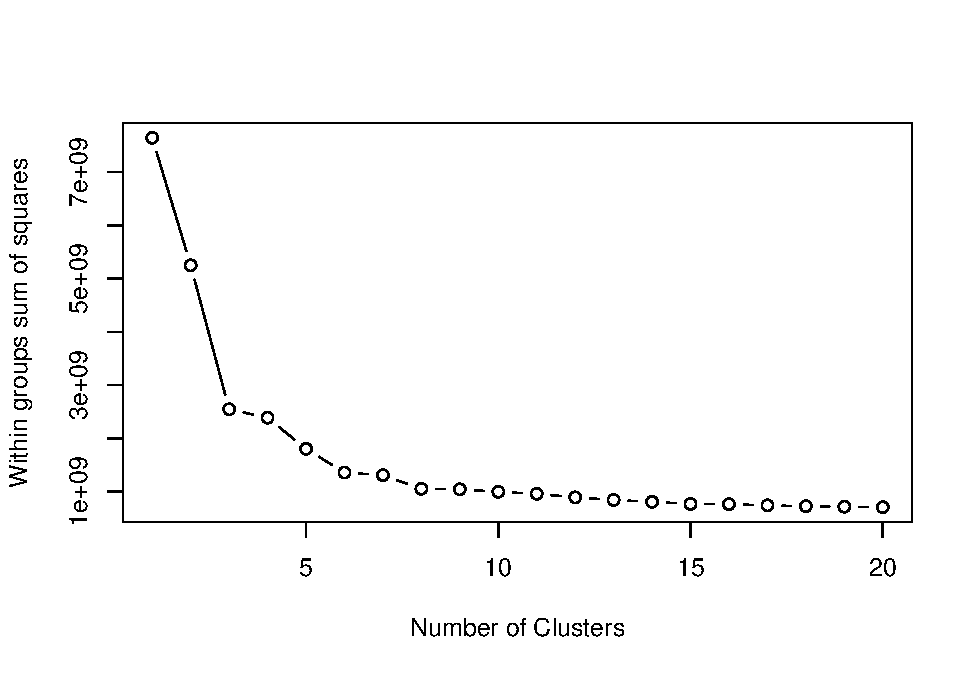
\includegraphics{Artificial-Stupidity_files/figure-latex/unnamed-chunk-20-1.pdf}

\begin{Shaded}
\begin{Highlighting}[]
\FunctionTok{set.seed}\NormalTok{(seed)}
\NormalTok{kc }\OtherTok{\textless{}{-}} \FunctionTok{kmeans}\NormalTok{(allData, }\AttributeTok{centers=}\DecValTok{15}\NormalTok{)}

\NormalTok{beforeCluster }\SpecialCharTok{\%\textgreater{}\%} \FunctionTok{mutate}\NormalTok{(}\AttributeTok{cluster =}\NormalTok{ kc}\SpecialCharTok{$}\NormalTok{cluster }\SpecialCharTok{\%\textgreater{}\%} \FunctionTok{as.factor}\NormalTok{()) }\OtherTok{{-}\textgreater{}}\NormalTok{ afterCluster}
\end{Highlighting}
\end{Shaded}

\hypertarget{generate-mean-price-for-clusters}{%
\paragraph{Generate mean price for
clusters}\label{generate-mean-price-for-clusters}}

Like mean price for areas, haveing the mean price for each cluster might
also help the model find the more appropreate price.

\begin{Shaded}
\begin{Highlighting}[]
\NormalTok{mean\_price\_cluster }\OtherTok{\textless{}{-}}\NormalTok{ afterCluster }\SpecialCharTok{\%\textgreater{}\%} 
  \FunctionTok{filter}\NormalTok{(price }\SpecialCharTok{\textgreater{}} \SpecialCharTok{{-}}\DecValTok{1}\NormalTok{) }\SpecialCharTok{\%\textgreater{}\%} 
  \FunctionTok{group\_by}\NormalTok{(}\AttributeTok{cluster =}\NormalTok{ cluster) }\SpecialCharTok{\%\textgreater{}\%}
  \FunctionTok{summarize}\NormalTok{(}\AttributeTok{price\_mean\_clus =} \FunctionTok{mean}\NormalTok{(price))}

\NormalTok{afterCluster }\OtherTok{\textless{}{-}}\NormalTok{ afterCluster }\SpecialCharTok{\%\textgreater{}\%} \FunctionTok{left\_join}\NormalTok{(mean\_price\_cluster, }\AttributeTok{by =} \FunctionTok{c}\NormalTok{(}\StringTok{"cluster"} \OtherTok{=} \StringTok{"cluster"}\NormalTok{))}

\CommentTok{\# plotting each cluster\textquotesingle{}s price distribution }
\NormalTok{pp }\OtherTok{\textless{}{-}}\NormalTok{ afterCluster }\SpecialCharTok{\%\textgreater{}\%} \FunctionTok{select}\NormalTok{(}\FunctionTok{c}\NormalTok{(price, cluster)) }\SpecialCharTok{\%\textgreater{}\%} \FunctionTok{ggplot}\NormalTok{(}\FunctionTok{aes}\NormalTok{(}\AttributeTok{x =}\NormalTok{ price, }\AttributeTok{color =}\NormalTok{ cluster)) }\SpecialCharTok{+} \FunctionTok{geom\_density}\NormalTok{()}
\NormalTok{pp }\SpecialCharTok{\%\textgreater{}\%} \FunctionTok{ggplotly}\NormalTok{()}
\end{Highlighting}
\end{Shaded}

\includegraphics{Artificial-Stupidity_files/figure-latex/unnamed-chunk-21-1.pdf}

\begin{Shaded}
\begin{Highlighting}[]
\NormalTok{allData }\OtherTok{\textless{}{-}}\NormalTok{ afterCluster }\SpecialCharTok{\%\textgreater{}\%} \FunctionTok{mutate}\NormalTok{(}\AttributeTok{cluster =}\NormalTok{ cluster }\SpecialCharTok{\%\textgreater{}\%} \FunctionTok{as.numeric}\NormalTok{())}
\end{Highlighting}
\end{Shaded}

\hypertarget{prepare-for-modeling}{%
\subsubsection{Prepare for modeling}\label{prepare-for-modeling}}

After all data are being cleaned, pre-processed, and transformed, we
need to prep it for modeling.

\hypertarget{separate-train-and-test}{%
\paragraph{Separate Train and Test}\label{separate-train-and-test}}

Training set and testing set are separated.

\begin{Shaded}
\begin{Highlighting}[]
\NormalTok{trainData }\OtherTok{\textless{}{-}}\NormalTok{ allData }\SpecialCharTok{\%\textgreater{}\%}
    \FunctionTok{select}\NormalTok{(}\SpecialCharTok{!}\NormalTok{is.character) }\SpecialCharTok{\%\textgreater{}\%} 
    \FunctionTok{filter}\NormalTok{(price }\SpecialCharTok{\textgreater{}} \SpecialCharTok{{-}}\DecValTok{1}\NormalTok{) }
\NormalTok{testData }\OtherTok{\textless{}{-}}\NormalTok{ allData }\SpecialCharTok{\%\textgreater{}\%}
    \FunctionTok{select}\NormalTok{(}\SpecialCharTok{!}\NormalTok{is.character) }\SpecialCharTok{\%\textgreater{}\%} 
    \FunctionTok{filter}\NormalTok{(price }\SpecialCharTok{==} \SpecialCharTok{{-}}\DecValTok{1}\NormalTok{) }\SpecialCharTok{\%\textgreater{}\%} \FunctionTok{select}\NormalTok{(}\SpecialCharTok{{-}}\NormalTok{price)}
\end{Highlighting}
\end{Shaded}

\hypertarget{feature-selection}{%
\paragraph{Feature selection}\label{feature-selection}}

To lighten the load of some models, we can perform a feature selection
on our data set. Some models might even perform better with less model.
The following code uses boruta algorithm, a tree based model, to
calculate feature importance.

\begin{Shaded}
\begin{Highlighting}[]
\NormalTok{boruta\_output }\OtherTok{\textless{}{-}}
  \FunctionTok{Boruta}\NormalTok{(}
\NormalTok{    price }\SpecialCharTok{\textasciitilde{}}\NormalTok{ .,}
    \AttributeTok{data =}\NormalTok{ trainData,}
    \AttributeTok{pValue =} \FloatTok{0.05}\NormalTok{,}
    \AttributeTok{maxRuns =} \DecValTok{500}\NormalTok{,}
    \AttributeTok{doTrace =} \DecValTok{2}\NormalTok{,}
    \AttributeTok{getImp =}\NormalTok{ getImpXgboost, }\CommentTok{\# delete this line for better result, keep it for faster output}
    \AttributeTok{nthread=}\NormalTok{cores,}
\NormalTok{  )}
\end{Highlighting}
\end{Shaded}

\begin{verbatim}
##  1. run of importance source...
\end{verbatim}

\begin{verbatim}
##  2. run of importance source...
\end{verbatim}

\begin{verbatim}
##  3. run of importance source...
\end{verbatim}

\begin{verbatim}
##  4. run of importance source...
\end{verbatim}

\begin{verbatim}
##  5. run of importance source...
\end{verbatim}

\begin{verbatim}
##  6. run of importance source...
\end{verbatim}

\begin{verbatim}
##  7. run of importance source...
\end{verbatim}

\begin{verbatim}
##  8. run of importance source...
\end{verbatim}

\begin{verbatim}
##  9. run of importance source...
\end{verbatim}

\begin{verbatim}
##  10. run of importance source...
\end{verbatim}

\begin{verbatim}
##  11. run of importance source...
\end{verbatim}

\begin{verbatim}
##  12. run of importance source...
\end{verbatim}

\begin{verbatim}
##  13. run of importance source...
\end{verbatim}

\begin{verbatim}
##  14. run of importance source...
\end{verbatim}

\begin{verbatim}
##  15. run of importance source...
\end{verbatim}

\begin{verbatim}
## After 15 iterations, +3.4 mins:
\end{verbatim}

\begin{verbatim}
##  confirmed 16 attributes: accommodates, availability_365, bathrooms, bedrooms, calculated_host_listings_count and 11 more;
\end{verbatim}

\begin{verbatim}
##  rejected 1025 attributes: accessible_height_bed_amen, accessible_height_toilet_amen, accommodates_2pow, accommodates_3pow, AdminName2 and 1020 more;
\end{verbatim}

\begin{verbatim}
##  still have 23 attributes left.
\end{verbatim}

\begin{verbatim}
##  16. run of importance source...
\end{verbatim}

\begin{verbatim}
##  17. run of importance source...
\end{verbatim}

\begin{verbatim}
##  18. run of importance source...
\end{verbatim}

\begin{verbatim}
##  19. run of importance source...
\end{verbatim}

\begin{verbatim}
## After 19 iterations, +3.5 mins:
\end{verbatim}

\begin{verbatim}
##  rejected 3 attributes: building_staff_amen, w156_2pow, w46;
\end{verbatim}

\begin{verbatim}
##  still have 20 attributes left.
\end{verbatim}

\begin{verbatim}
##  20. run of importance source...
\end{verbatim}

\begin{verbatim}
##  21. run of importance source...
\end{verbatim}

\begin{verbatim}
##  22. run of importance source...
\end{verbatim}

\begin{verbatim}
##  23. run of importance source...
\end{verbatim}

\begin{verbatim}
## After 23 iterations, +3.5 mins:
\end{verbatim}

\begin{verbatim}
##  confirmed 1 attribute: w171;
\end{verbatim}

\begin{verbatim}
##  rejected 1 attribute: heating_amen;
\end{verbatim}

\begin{verbatim}
##  still have 18 attributes left.
\end{verbatim}

\begin{verbatim}
##  24. run of importance source...
\end{verbatim}

\begin{verbatim}
##  25. run of importance source...
\end{verbatim}

\begin{verbatim}
##  26. run of importance source...
\end{verbatim}

\begin{verbatim}
## After 26 iterations, +3.5 mins:
\end{verbatim}

\begin{verbatim}
##  rejected 1 attribute: n_chars;
\end{verbatim}

\begin{verbatim}
##  still have 17 attributes left.
\end{verbatim}

\begin{verbatim}
##  27. run of importance source...
\end{verbatim}

\begin{verbatim}
##  28. run of importance source...
\end{verbatim}

\begin{verbatim}
##  29. run of importance source...
\end{verbatim}

\begin{verbatim}
##  30. run of importance source...
\end{verbatim}

\begin{verbatim}
##  31. run of importance source...
\end{verbatim}

\begin{verbatim}
##  32. run of importance source...
\end{verbatim}

\begin{verbatim}
##  33. run of importance source...
\end{verbatim}

\begin{verbatim}
##  34. run of importance source...
\end{verbatim}

\begin{verbatim}
##  35. run of importance source...
\end{verbatim}

\begin{verbatim}
##  36. run of importance source...
\end{verbatim}

\begin{verbatim}
##  37. run of importance source...
\end{verbatim}

\begin{verbatim}
##  38. run of importance source...
\end{verbatim}

\begin{verbatim}
##  39. run of importance source...
\end{verbatim}

\begin{verbatim}
##  40. run of importance source...
\end{verbatim}

\begin{verbatim}
##  41. run of importance source...
\end{verbatim}

\begin{verbatim}
##  42. run of importance source...
\end{verbatim}

\begin{verbatim}
## After 42 iterations, +3.6 mins:
\end{verbatim}

\begin{verbatim}
##  confirmed 1 attribute: host_since;
\end{verbatim}

\begin{verbatim}
##  still have 16 attributes left.
\end{verbatim}

\begin{verbatim}
##  43. run of importance source...
\end{verbatim}

\begin{verbatim}
##  44. run of importance source...
\end{verbatim}

\begin{verbatim}
##  45. run of importance source...
\end{verbatim}

\begin{verbatim}
##  46. run of importance source...
\end{verbatim}

\begin{verbatim}
##  47. run of importance source...
\end{verbatim}

\begin{verbatim}
##  48. run of importance source...
\end{verbatim}

\begin{verbatim}
## After 48 iterations, +3.7 mins:
\end{verbatim}

\begin{verbatim}
##  confirmed 1 attribute: w20;
\end{verbatim}

\begin{verbatim}
##  still have 15 attributes left.
\end{verbatim}

\begin{verbatim}
##  49. run of importance source...
\end{verbatim}

\begin{verbatim}
##  50. run of importance source...
\end{verbatim}

\begin{verbatim}
##  51. run of importance source...
\end{verbatim}

\begin{verbatim}
##  52. run of importance source...
\end{verbatim}

\begin{verbatim}
##  53. run of importance source...
\end{verbatim}

\begin{verbatim}
##  54. run of importance source...
\end{verbatim}

\begin{verbatim}
##  55. run of importance source...
\end{verbatim}

\begin{verbatim}
##  56. run of importance source...
\end{verbatim}

\begin{verbatim}
## After 56 iterations, +3.7 mins:
\end{verbatim}

\begin{verbatim}
##  confirmed 1 attribute: minimum_minimum_nights;
\end{verbatim}

\begin{verbatim}
##  still have 14 attributes left.
\end{verbatim}

\begin{verbatim}
##  57. run of importance source...
\end{verbatim}

\begin{verbatim}
##  58. run of importance source...
\end{verbatim}

\begin{verbatim}
##  59. run of importance source...
\end{verbatim}

\begin{verbatim}
##  60. run of importance source...
\end{verbatim}

\begin{verbatim}
##  61. run of importance source...
\end{verbatim}

\begin{verbatim}
##  62. run of importance source...
\end{verbatim}

\begin{verbatim}
##  63. run of importance source...
\end{verbatim}

\begin{verbatim}
##  64. run of importance source...
\end{verbatim}

\begin{verbatim}
##  65. run of importance source...
\end{verbatim}

\begin{verbatim}
##  66. run of importance source...
\end{verbatim}

\begin{verbatim}
##  67. run of importance source...
\end{verbatim}

\begin{verbatim}
## After 67 iterations, +3.8 mins:
\end{verbatim}

\begin{verbatim}
##  confirmed 1 attribute: availability_60;
\end{verbatim}

\begin{verbatim}
##  still have 13 attributes left.
\end{verbatim}

\begin{verbatim}
##  68. run of importance source...
\end{verbatim}

\begin{verbatim}
##  69. run of importance source...
\end{verbatim}

\begin{verbatim}
## After 69 iterations, +3.8 mins:
\end{verbatim}

\begin{verbatim}
##  confirmed 1 attribute: security_deposit;
\end{verbatim}

\begin{verbatim}
##  still have 12 attributes left.
\end{verbatim}

\begin{verbatim}
##  70. run of importance source...
\end{verbatim}

\begin{verbatim}
##  71. run of importance source...
\end{verbatim}

\begin{verbatim}
##  72. run of importance source...
\end{verbatim}

\begin{verbatim}
## After 72 iterations, +3.9 mins:
\end{verbatim}

\begin{verbatim}
##  confirmed 2 attributes: w150, zipcode;
\end{verbatim}

\begin{verbatim}
##  still have 10 attributes left.
\end{verbatim}

\begin{verbatim}
##  73. run of importance source...
\end{verbatim}

\begin{verbatim}
##  74. run of importance source...
\end{verbatim}

\begin{verbatim}
##  75. run of importance source...
\end{verbatim}

\begin{verbatim}
##  76. run of importance source...
\end{verbatim}

\begin{verbatim}
##  77. run of importance source...
\end{verbatim}

\begin{verbatim}
##  78. run of importance source...
\end{verbatim}

\begin{verbatim}
##  79. run of importance source...
\end{verbatim}

\begin{verbatim}
##  80. run of importance source...
\end{verbatim}

\begin{verbatim}
##  81. run of importance source...
\end{verbatim}

\begin{verbatim}
##  82. run of importance source...
\end{verbatim}

\begin{verbatim}
##  83. run of importance source...
\end{verbatim}

\begin{verbatim}
##  84. run of importance source...
\end{verbatim}

\begin{verbatim}
##  85. run of importance source...
\end{verbatim}

\begin{verbatim}
##  86. run of importance source...
\end{verbatim}

\begin{verbatim}
##  87. run of importance source...
\end{verbatim}

\begin{verbatim}
## After 87 iterations, +4 mins:
\end{verbatim}

\begin{verbatim}
##  confirmed 2 attributes: first_review, n_nonasciis;
\end{verbatim}

\begin{verbatim}
##  still have 8 attributes left.
\end{verbatim}

\begin{verbatim}
##  88. run of importance source...
\end{verbatim}

\begin{verbatim}
##  89. run of importance source...
\end{verbatim}

\begin{verbatim}
##  90. run of importance source...
\end{verbatim}

\begin{verbatim}
##  91. run of importance source...
\end{verbatim}

\begin{verbatim}
##  92. run of importance source...
\end{verbatim}

\begin{verbatim}
##  93. run of importance source...
\end{verbatim}

\begin{verbatim}
##  94. run of importance source...
\end{verbatim}

\begin{verbatim}
##  95. run of importance source...
\end{verbatim}

\begin{verbatim}
##  96. run of importance source...
\end{verbatim}

\begin{verbatim}
##  97. run of importance source...
\end{verbatim}

\begin{verbatim}
##  98. run of importance source...
\end{verbatim}

\begin{verbatim}
##  99. run of importance source...
\end{verbatim}

\begin{verbatim}
##  100. run of importance source...
\end{verbatim}

\begin{verbatim}
##  101. run of importance source...
\end{verbatim}

\begin{verbatim}
##  102. run of importance source...
\end{verbatim}

\begin{verbatim}
##  103. run of importance source...
\end{verbatim}

\begin{verbatim}
##  104. run of importance source...
\end{verbatim}

\begin{verbatim}
##  105. run of importance source...
\end{verbatim}

\begin{verbatim}
##  106. run of importance source...
\end{verbatim}

\begin{verbatim}
##  107. run of importance source...
\end{verbatim}

\begin{verbatim}
##  108. run of importance source...
\end{verbatim}

\begin{verbatim}
##  109. run of importance source...
\end{verbatim}

\begin{verbatim}
##  110. run of importance source...
\end{verbatim}

\begin{verbatim}
##  111. run of importance source...
\end{verbatim}

\begin{verbatim}
##  112. run of importance source...
\end{verbatim}

\begin{verbatim}
##  113. run of importance source...
\end{verbatim}

\begin{verbatim}
##  114. run of importance source...
\end{verbatim}

\begin{verbatim}
##  115. run of importance source...
\end{verbatim}

\begin{verbatim}
##  116. run of importance source...
\end{verbatim}

\begin{verbatim}
##  117. run of importance source...
\end{verbatim}

\begin{verbatim}
##  118. run of importance source...
\end{verbatim}

\begin{verbatim}
##  119. run of importance source...
\end{verbatim}

\begin{verbatim}
##  120. run of importance source...
\end{verbatim}

\begin{verbatim}
## After 120 iterations, +4.2 mins:
\end{verbatim}

\begin{verbatim}
##  confirmed 1 attribute: n_commas;
\end{verbatim}

\begin{verbatim}
##  still have 7 attributes left.
\end{verbatim}

\begin{verbatim}
##  121. run of importance source...
\end{verbatim}

\begin{verbatim}
##  122. run of importance source...
\end{verbatim}

\begin{verbatim}
##  123. run of importance source...
\end{verbatim}

\begin{verbatim}
##  124. run of importance source...
\end{verbatim}

\begin{verbatim}
##  125. run of importance source...
\end{verbatim}

\begin{verbatim}
##  126. run of importance source...
\end{verbatim}

\begin{verbatim}
##  127. run of importance source...
\end{verbatim}

\begin{verbatim}
##  128. run of importance source...
\end{verbatim}

\begin{verbatim}
##  129. run of importance source...
\end{verbatim}

\begin{verbatim}
##  130. run of importance source...
\end{verbatim}

\begin{verbatim}
##  131. run of importance source...
\end{verbatim}

\begin{verbatim}
##  132. run of importance source...
\end{verbatim}

\begin{verbatim}
## After 132 iterations, +4.3 mins:
\end{verbatim}

\begin{verbatim}
##  confirmed 1 attribute: w47;
\end{verbatim}

\begin{verbatim}
##  still have 6 attributes left.
\end{verbatim}

\begin{verbatim}
##  133. run of importance source...
\end{verbatim}

\begin{verbatim}
##  134. run of importance source...
\end{verbatim}

\begin{verbatim}
##  135. run of importance source...
\end{verbatim}

\begin{verbatim}
##  136. run of importance source...
\end{verbatim}

\begin{verbatim}
##  137. run of importance source...
\end{verbatim}

\begin{verbatim}
##  138. run of importance source...
\end{verbatim}

\begin{verbatim}
##  139. run of importance source...
\end{verbatim}

\begin{verbatim}
##  140. run of importance source...
\end{verbatim}

\begin{verbatim}
##  141. run of importance source...
\end{verbatim}

\begin{verbatim}
##  142. run of importance source...
\end{verbatim}

\begin{verbatim}
##  143. run of importance source...
\end{verbatim}

\begin{verbatim}
##  144. run of importance source...
\end{verbatim}

\begin{verbatim}
##  145. run of importance source...
\end{verbatim}

\begin{verbatim}
##  146. run of importance source...
\end{verbatim}

\begin{verbatim}
##  147. run of importance source...
\end{verbatim}

\begin{verbatim}
##  148. run of importance source...
\end{verbatim}

\begin{verbatim}
##  149. run of importance source...
\end{verbatim}

\begin{verbatim}
##  150. run of importance source...
\end{verbatim}

\begin{verbatim}
##  151. run of importance source...
\end{verbatim}

\begin{verbatim}
##  152. run of importance source...
\end{verbatim}

\begin{verbatim}
##  153. run of importance source...
\end{verbatim}

\begin{verbatim}
##  154. run of importance source...
\end{verbatim}

\begin{verbatim}
##  155. run of importance source...
\end{verbatim}

\begin{verbatim}
##  156. run of importance source...
\end{verbatim}

\begin{verbatim}
##  157. run of importance source...
\end{verbatim}

\begin{verbatim}
##  158. run of importance source...
\end{verbatim}

\begin{verbatim}
##  159. run of importance source...
\end{verbatim}

\begin{verbatim}
##  160. run of importance source...
\end{verbatim}

\begin{verbatim}
##  161. run of importance source...
\end{verbatim}

\begin{verbatim}
## After 161 iterations, +4.5 mins:
\end{verbatim}

\begin{verbatim}
##  confirmed 1 attribute: w117;
\end{verbatim}

\begin{verbatim}
##  still have 5 attributes left.
\end{verbatim}

\begin{verbatim}
##  162. run of importance source...
\end{verbatim}

\begin{verbatim}
##  163. run of importance source...
\end{verbatim}

\begin{verbatim}
##  164. run of importance source...
\end{verbatim}

\begin{verbatim}
##  165. run of importance source...
\end{verbatim}

\begin{verbatim}
##  166. run of importance source...
\end{verbatim}

\begin{verbatim}
##  167. run of importance source...
\end{verbatim}

\begin{verbatim}
##  168. run of importance source...
\end{verbatim}

\begin{verbatim}
##  169. run of importance source...
\end{verbatim}

\begin{verbatim}
##  170. run of importance source...
\end{verbatim}

\begin{verbatim}
##  171. run of importance source...
\end{verbatim}

\begin{verbatim}
##  172. run of importance source...
\end{verbatim}

\begin{verbatim}
##  173. run of importance source...
\end{verbatim}

\begin{verbatim}
##  174. run of importance source...
\end{verbatim}

\begin{verbatim}
##  175. run of importance source...
\end{verbatim}

\begin{verbatim}
##  176. run of importance source...
\end{verbatim}

\begin{verbatim}
##  177. run of importance source...
\end{verbatim}

\begin{verbatim}
##  178. run of importance source...
\end{verbatim}

\begin{verbatim}
##  179. run of importance source...
\end{verbatim}

\begin{verbatim}
##  180. run of importance source...
\end{verbatim}

\begin{verbatim}
##  181. run of importance source...
\end{verbatim}

\begin{verbatim}
##  182. run of importance source...
\end{verbatim}

\begin{verbatim}
##  183. run of importance source...
\end{verbatim}

\begin{verbatim}
##  184. run of importance source...
\end{verbatim}

\begin{verbatim}
##  185. run of importance source...
\end{verbatim}

\begin{verbatim}
##  186. run of importance source...
\end{verbatim}

\begin{verbatim}
##  187. run of importance source...
\end{verbatim}

\begin{verbatim}
##  188. run of importance source...
\end{verbatim}

\begin{verbatim}
##  189. run of importance source...
\end{verbatim}

\begin{verbatim}
##  190. run of importance source...
\end{verbatim}

\begin{verbatim}
##  191. run of importance source...
\end{verbatim}

\begin{verbatim}
##  192. run of importance source...
\end{verbatim}

\begin{verbatim}
##  193. run of importance source...
\end{verbatim}

\begin{verbatim}
##  194. run of importance source...
\end{verbatim}

\begin{verbatim}
##  195. run of importance source...
\end{verbatim}

\begin{verbatim}
##  196. run of importance source...
\end{verbatim}

\begin{verbatim}
##  197. run of importance source...
\end{verbatim}

\begin{verbatim}
##  198. run of importance source...
\end{verbatim}

\begin{verbatim}
##  199. run of importance source...
\end{verbatim}

\begin{verbatim}
##  200. run of importance source...
\end{verbatim}

\begin{verbatim}
##  201. run of importance source...
\end{verbatim}

\begin{verbatim}
##  202. run of importance source...
\end{verbatim}

\begin{verbatim}
##  203. run of importance source...
\end{verbatim}

\begin{verbatim}
##  204. run of importance source...
\end{verbatim}

\begin{verbatim}
##  205. run of importance source...
\end{verbatim}

\begin{verbatim}
##  206. run of importance source...
\end{verbatim}

\begin{verbatim}
##  207. run of importance source...
\end{verbatim}

\begin{verbatim}
##  208. run of importance source...
\end{verbatim}

\begin{verbatim}
##  209. run of importance source...
\end{verbatim}

\begin{verbatim}
##  210. run of importance source...
\end{verbatim}

\begin{verbatim}
##  211. run of importance source...
\end{verbatim}

\begin{verbatim}
##  212. run of importance source...
\end{verbatim}

\begin{verbatim}
##  213. run of importance source...
\end{verbatim}

\begin{verbatim}
##  214. run of importance source...
\end{verbatim}

\begin{verbatim}
##  215. run of importance source...
\end{verbatim}

\begin{verbatim}
##  216. run of importance source...
\end{verbatim}

\begin{verbatim}
##  217. run of importance source...
\end{verbatim}

\begin{verbatim}
##  218. run of importance source...
\end{verbatim}

\begin{verbatim}
##  219. run of importance source...
\end{verbatim}

\begin{verbatim}
##  220. run of importance source...
\end{verbatim}

\begin{verbatim}
##  221. run of importance source...
\end{verbatim}

\begin{verbatim}
##  222. run of importance source...
\end{verbatim}

\begin{verbatim}
##  223. run of importance source...
\end{verbatim}

\begin{verbatim}
##  224. run of importance source...
\end{verbatim}

\begin{verbatim}
##  225. run of importance source...
\end{verbatim}

\begin{verbatim}
##  226. run of importance source...
\end{verbatim}

\begin{verbatim}
##  227. run of importance source...
\end{verbatim}

\begin{verbatim}
##  228. run of importance source...
\end{verbatim}

\begin{verbatim}
##  229. run of importance source...
\end{verbatim}

\begin{verbatim}
##  230. run of importance source...
\end{verbatim}

\begin{verbatim}
##  231. run of importance source...
\end{verbatim}

\begin{verbatim}
##  232. run of importance source...
\end{verbatim}

\begin{verbatim}
##  233. run of importance source...
\end{verbatim}

\begin{verbatim}
##  234. run of importance source...
\end{verbatim}

\begin{verbatim}
##  235. run of importance source...
\end{verbatim}

\begin{verbatim}
##  236. run of importance source...
\end{verbatim}

\begin{verbatim}
##  237. run of importance source...
\end{verbatim}

\begin{verbatim}
##  238. run of importance source...
\end{verbatim}

\begin{verbatim}
##  239. run of importance source...
\end{verbatim}

\begin{verbatim}
##  240. run of importance source...
\end{verbatim}

\begin{verbatim}
##  241. run of importance source...
\end{verbatim}

\begin{verbatim}
##  242. run of importance source...
\end{verbatim}

\begin{verbatim}
##  243. run of importance source...
\end{verbatim}

\begin{verbatim}
##  244. run of importance source...
\end{verbatim}

\begin{verbatim}
##  245. run of importance source...
\end{verbatim}

\begin{verbatim}
##  246. run of importance source...
\end{verbatim}

\begin{verbatim}
##  247. run of importance source...
\end{verbatim}

\begin{verbatim}
##  248. run of importance source...
\end{verbatim}

\begin{verbatim}
##  249. run of importance source...
\end{verbatim}

\begin{verbatim}
##  250. run of importance source...
\end{verbatim}

\begin{verbatim}
##  251. run of importance source...
\end{verbatim}

\begin{verbatim}
##  252. run of importance source...
\end{verbatim}

\begin{verbatim}
##  253. run of importance source...
\end{verbatim}

\begin{verbatim}
##  254. run of importance source...
\end{verbatim}

\begin{verbatim}
##  255. run of importance source...
\end{verbatim}

\begin{verbatim}
##  256. run of importance source...
\end{verbatim}

\begin{verbatim}
##  257. run of importance source...
\end{verbatim}

\begin{verbatim}
##  258. run of importance source...
\end{verbatim}

\begin{verbatim}
##  259. run of importance source...
\end{verbatim}

\begin{verbatim}
##  260. run of importance source...
\end{verbatim}

\begin{verbatim}
##  261. run of importance source...
\end{verbatim}

\begin{verbatim}
##  262. run of importance source...
\end{verbatim}

\begin{verbatim}
##  263. run of importance source...
\end{verbatim}

\begin{verbatim}
##  264. run of importance source...
\end{verbatim}

\begin{verbatim}
##  265. run of importance source...
\end{verbatim}

\begin{verbatim}
##  266. run of importance source...
\end{verbatim}

\begin{verbatim}
##  267. run of importance source...
\end{verbatim}

\begin{verbatim}
##  268. run of importance source...
\end{verbatim}

\begin{verbatim}
##  269. run of importance source...
\end{verbatim}

\begin{verbatim}
##  270. run of importance source...
\end{verbatim}

\begin{verbatim}
##  271. run of importance source...
\end{verbatim}

\begin{verbatim}
##  272. run of importance source...
\end{verbatim}

\begin{verbatim}
##  273. run of importance source...
\end{verbatim}

\begin{verbatim}
##  274. run of importance source...
\end{verbatim}

\begin{verbatim}
##  275. run of importance source...
\end{verbatim}

\begin{verbatim}
##  276. run of importance source...
\end{verbatim}

\begin{verbatim}
##  277. run of importance source...
\end{verbatim}

\begin{verbatim}
##  278. run of importance source...
\end{verbatim}

\begin{verbatim}
## After 278 iterations, +5.3 mins:
\end{verbatim}

\begin{verbatim}
##  confirmed 1 attribute: availability_90;
\end{verbatim}

\begin{verbatim}
##  still have 4 attributes left.
\end{verbatim}

\begin{verbatim}
##  279. run of importance source...
\end{verbatim}

\begin{verbatim}
##  280. run of importance source...
\end{verbatim}

\begin{verbatim}
##  281. run of importance source...
\end{verbatim}

\begin{verbatim}
##  282. run of importance source...
\end{verbatim}

\begin{verbatim}
##  283. run of importance source...
\end{verbatim}

\begin{verbatim}
##  284. run of importance source...
\end{verbatim}

\begin{verbatim}
##  285. run of importance source...
\end{verbatim}

\begin{verbatim}
##  286. run of importance source...
\end{verbatim}

\begin{verbatim}
##  287. run of importance source...
\end{verbatim}

\begin{verbatim}
##  288. run of importance source...
\end{verbatim}

\begin{verbatim}
##  289. run of importance source...
\end{verbatim}

\begin{verbatim}
##  290. run of importance source...
\end{verbatim}

\begin{verbatim}
##  291. run of importance source...
\end{verbatim}

\begin{verbatim}
##  292. run of importance source...
\end{verbatim}

\begin{verbatim}
##  293. run of importance source...
\end{verbatim}

\begin{verbatim}
##  294. run of importance source...
\end{verbatim}

\begin{verbatim}
##  295. run of importance source...
\end{verbatim}

\begin{verbatim}
##  296. run of importance source...
\end{verbatim}

\begin{verbatim}
##  297. run of importance source...
\end{verbatim}

\begin{verbatim}
##  298. run of importance source...
\end{verbatim}

\begin{verbatim}
##  299. run of importance source...
\end{verbatim}

\begin{verbatim}
##  300. run of importance source...
\end{verbatim}

\begin{verbatim}
##  301. run of importance source...
\end{verbatim}

\begin{verbatim}
##  302. run of importance source...
\end{verbatim}

\begin{verbatim}
##  303. run of importance source...
\end{verbatim}

\begin{verbatim}
##  304. run of importance source...
\end{verbatim}

\begin{verbatim}
##  305. run of importance source...
\end{verbatim}

\begin{verbatim}
##  306. run of importance source...
\end{verbatim}

\begin{verbatim}
##  307. run of importance source...
\end{verbatim}

\begin{verbatim}
##  308. run of importance source...
\end{verbatim}

\begin{verbatim}
##  309. run of importance source...
\end{verbatim}

\begin{verbatim}
##  310. run of importance source...
\end{verbatim}

\begin{verbatim}
## After 310 iterations, +5.6 mins:
\end{verbatim}

\begin{verbatim}
##  confirmed 1 attribute: record_count_c;
\end{verbatim}

\begin{verbatim}
##  still have 3 attributes left.
\end{verbatim}

\begin{verbatim}
##  311. run of importance source...
\end{verbatim}

\begin{verbatim}
##  312. run of importance source...
\end{verbatim}

\begin{verbatim}
##  313. run of importance source...
\end{verbatim}

\begin{verbatim}
##  314. run of importance source...
\end{verbatim}

\begin{verbatim}
##  315. run of importance source...
\end{verbatim}

\begin{verbatim}
##  316. run of importance source...
\end{verbatim}

\begin{verbatim}
##  317. run of importance source...
\end{verbatim}

\begin{verbatim}
##  318. run of importance source...
\end{verbatim}

\begin{verbatim}
##  319. run of importance source...
\end{verbatim}

\begin{verbatim}
##  320. run of importance source...
\end{verbatim}

\begin{verbatim}
##  321. run of importance source...
\end{verbatim}

\begin{verbatim}
##  322. run of importance source...
\end{verbatim}

\begin{verbatim}
##  323. run of importance source...
\end{verbatim}

\begin{verbatim}
##  324. run of importance source...
\end{verbatim}

\begin{verbatim}
##  325. run of importance source...
\end{verbatim}

\begin{verbatim}
##  326. run of importance source...
\end{verbatim}

\begin{verbatim}
##  327. run of importance source...
\end{verbatim}

\begin{verbatim}
##  328. run of importance source...
\end{verbatim}

\begin{verbatim}
##  329. run of importance source...
\end{verbatim}

\begin{verbatim}
##  330. run of importance source...
\end{verbatim}

\begin{verbatim}
##  331. run of importance source...
\end{verbatim}

\begin{verbatim}
##  332. run of importance source...
\end{verbatim}

\begin{verbatim}
##  333. run of importance source...
\end{verbatim}

\begin{verbatim}
##  334. run of importance source...
\end{verbatim}

\begin{verbatim}
##  335. run of importance source...
\end{verbatim}

\begin{verbatim}
##  336. run of importance source...
\end{verbatim}

\begin{verbatim}
##  337. run of importance source...
\end{verbatim}

\begin{verbatim}
##  338. run of importance source...
\end{verbatim}

\begin{verbatim}
##  339. run of importance source...
\end{verbatim}

\begin{verbatim}
##  340. run of importance source...
\end{verbatim}

\begin{verbatim}
##  341. run of importance source...
\end{verbatim}

\begin{verbatim}
##  342. run of importance source...
\end{verbatim}

\begin{verbatim}
##  343. run of importance source...
\end{verbatim}

\begin{verbatim}
##  344. run of importance source...
\end{verbatim}

\begin{verbatim}
##  345. run of importance source...
\end{verbatim}

\begin{verbatim}
##  346. run of importance source...
\end{verbatim}

\begin{verbatim}
##  347. run of importance source...
\end{verbatim}

\begin{verbatim}
##  348. run of importance source...
\end{verbatim}

\begin{verbatim}
##  349. run of importance source...
\end{verbatim}

\begin{verbatim}
##  350. run of importance source...
\end{verbatim}

\begin{verbatim}
##  351. run of importance source...
\end{verbatim}

\begin{verbatim}
##  352. run of importance source...
\end{verbatim}

\begin{verbatim}
##  353. run of importance source...
\end{verbatim}

\begin{verbatim}
##  354. run of importance source...
\end{verbatim}

\begin{verbatim}
##  355. run of importance source...
\end{verbatim}

\begin{verbatim}
##  356. run of importance source...
\end{verbatim}

\begin{verbatim}
##  357. run of importance source...
\end{verbatim}

\begin{verbatim}
##  358. run of importance source...
\end{verbatim}

\begin{verbatim}
##  359. run of importance source...
\end{verbatim}

\begin{verbatim}
##  360. run of importance source...
\end{verbatim}

\begin{verbatim}
##  361. run of importance source...
\end{verbatim}

\begin{verbatim}
##  362. run of importance source...
\end{verbatim}

\begin{verbatim}
##  363. run of importance source...
\end{verbatim}

\begin{verbatim}
##  364. run of importance source...
\end{verbatim}

\begin{verbatim}
##  365. run of importance source...
\end{verbatim}

\begin{verbatim}
##  366. run of importance source...
\end{verbatim}

\begin{verbatim}
##  367. run of importance source...
\end{verbatim}

\begin{verbatim}
##  368. run of importance source...
\end{verbatim}

\begin{verbatim}
##  369. run of importance source...
\end{verbatim}

\begin{verbatim}
##  370. run of importance source...
\end{verbatim}

\begin{verbatim}
##  371. run of importance source...
\end{verbatim}

\begin{verbatim}
##  372. run of importance source...
\end{verbatim}

\begin{verbatim}
##  373. run of importance source...
\end{verbatim}

\begin{verbatim}
##  374. run of importance source...
\end{verbatim}

\begin{verbatim}
##  375. run of importance source...
\end{verbatim}

\begin{verbatim}
##  376. run of importance source...
\end{verbatim}

\begin{verbatim}
##  377. run of importance source...
\end{verbatim}

\begin{verbatim}
##  378. run of importance source...
\end{verbatim}

\begin{verbatim}
##  379. run of importance source...
\end{verbatim}

\begin{verbatim}
##  380. run of importance source...
\end{verbatim}

\begin{verbatim}
##  381. run of importance source...
\end{verbatim}

\begin{verbatim}
##  382. run of importance source...
\end{verbatim}

\begin{verbatim}
##  383. run of importance source...
\end{verbatim}

\begin{verbatim}
##  384. run of importance source...
\end{verbatim}

\begin{verbatim}
##  385. run of importance source...
\end{verbatim}

\begin{verbatim}
##  386. run of importance source...
\end{verbatim}

\begin{verbatim}
##  387. run of importance source...
\end{verbatim}

\begin{verbatim}
##  388. run of importance source...
\end{verbatim}

\begin{verbatim}
##  389. run of importance source...
\end{verbatim}

\begin{verbatim}
##  390. run of importance source...
\end{verbatim}

\begin{verbatim}
##  391. run of importance source...
\end{verbatim}

\begin{verbatim}
##  392. run of importance source...
\end{verbatim}

\begin{verbatim}
##  393. run of importance source...
\end{verbatim}

\begin{verbatim}
##  394. run of importance source...
\end{verbatim}

\begin{verbatim}
##  395. run of importance source...
\end{verbatim}

\begin{verbatim}
##  396. run of importance source...
\end{verbatim}

\begin{verbatim}
##  397. run of importance source...
\end{verbatim}

\begin{verbatim}
##  398. run of importance source...
\end{verbatim}

\begin{verbatim}
##  399. run of importance source...
\end{verbatim}

\begin{verbatim}
##  400. run of importance source...
\end{verbatim}

\begin{verbatim}
##  401. run of importance source...
\end{verbatim}

\begin{verbatim}
##  402. run of importance source...
\end{verbatim}

\begin{verbatim}
##  403. run of importance source...
\end{verbatim}

\begin{verbatim}
##  404. run of importance source...
\end{verbatim}

\begin{verbatim}
##  405. run of importance source...
\end{verbatim}

\begin{verbatim}
##  406. run of importance source...
\end{verbatim}

\begin{verbatim}
##  407. run of importance source...
\end{verbatim}

\begin{verbatim}
##  408. run of importance source...
\end{verbatim}

\begin{verbatim}
##  409. run of importance source...
\end{verbatim}

\begin{verbatim}
##  410. run of importance source...
\end{verbatim}

\begin{verbatim}
##  411. run of importance source...
\end{verbatim}

\begin{verbatim}
##  412. run of importance source...
\end{verbatim}

\begin{verbatim}
##  413. run of importance source...
\end{verbatim}

\begin{verbatim}
##  414. run of importance source...
\end{verbatim}

\begin{verbatim}
##  415. run of importance source...
\end{verbatim}

\begin{verbatim}
##  416. run of importance source...
\end{verbatim}

\begin{verbatim}
##  417. run of importance source...
\end{verbatim}

\begin{verbatim}
##  418. run of importance source...
\end{verbatim}

\begin{verbatim}
##  419. run of importance source...
\end{verbatim}

\begin{verbatim}
## After 419 iterations, +6.4 mins:
\end{verbatim}

\begin{verbatim}
##  rejected 1 attribute: PlaceName;
\end{verbatim}

\begin{verbatim}
##  still have 2 attributes left.
\end{verbatim}

\begin{verbatim}
##  420. run of importance source...
\end{verbatim}

\begin{verbatim}
##  421. run of importance source...
\end{verbatim}

\begin{verbatim}
##  422. run of importance source...
\end{verbatim}

\begin{verbatim}
##  423. run of importance source...
\end{verbatim}

\begin{verbatim}
##  424. run of importance source...
\end{verbatim}

\begin{verbatim}
##  425. run of importance source...
\end{verbatim}

\begin{verbatim}
##  426. run of importance source...
\end{verbatim}

\begin{verbatim}
##  427. run of importance source...
\end{verbatim}

\begin{verbatim}
##  428. run of importance source...
\end{verbatim}

\begin{verbatim}
##  429. run of importance source...
\end{verbatim}

\begin{verbatim}
##  430. run of importance source...
\end{verbatim}

\begin{verbatim}
##  431. run of importance source...
\end{verbatim}

\begin{verbatim}
##  432. run of importance source...
\end{verbatim}

\begin{verbatim}
##  433. run of importance source...
\end{verbatim}

\begin{verbatim}
##  434. run of importance source...
\end{verbatim}

\begin{verbatim}
##  435. run of importance source...
\end{verbatim}

\begin{verbatim}
##  436. run of importance source...
\end{verbatim}

\begin{verbatim}
##  437. run of importance source...
\end{verbatim}

\begin{verbatim}
##  438. run of importance source...
\end{verbatim}

\begin{verbatim}
##  439. run of importance source...
\end{verbatim}

\begin{verbatim}
##  440. run of importance source...
\end{verbatim}

\begin{verbatim}
##  441. run of importance source...
\end{verbatim}

\begin{verbatim}
##  442. run of importance source...
\end{verbatim}

\begin{verbatim}
##  443. run of importance source...
\end{verbatim}

\begin{verbatim}
##  444. run of importance source...
\end{verbatim}

\begin{verbatim}
##  445. run of importance source...
\end{verbatim}

\begin{verbatim}
##  446. run of importance source...
\end{verbatim}

\begin{verbatim}
##  447. run of importance source...
\end{verbatim}

\begin{verbatim}
##  448. run of importance source...
\end{verbatim}

\begin{verbatim}
##  449. run of importance source...
\end{verbatim}

\begin{verbatim}
##  450. run of importance source...
\end{verbatim}

\begin{verbatim}
##  451. run of importance source...
\end{verbatim}

\begin{verbatim}
##  452. run of importance source...
\end{verbatim}

\begin{verbatim}
##  453. run of importance source...
\end{verbatim}

\begin{verbatim}
##  454. run of importance source...
\end{verbatim}

\begin{verbatim}
##  455. run of importance source...
\end{verbatim}

\begin{verbatim}
##  456. run of importance source...
\end{verbatim}

\begin{verbatim}
##  457. run of importance source...
\end{verbatim}

\begin{verbatim}
##  458. run of importance source...
\end{verbatim}

\begin{verbatim}
##  459. run of importance source...
\end{verbatim}

\begin{verbatim}
##  460. run of importance source...
\end{verbatim}

\begin{verbatim}
##  461. run of importance source...
\end{verbatim}

\begin{verbatim}
##  462. run of importance source...
\end{verbatim}

\begin{verbatim}
##  463. run of importance source...
\end{verbatim}

\begin{verbatim}
##  464. run of importance source...
\end{verbatim}

\begin{verbatim}
##  465. run of importance source...
\end{verbatim}

\begin{verbatim}
##  466. run of importance source...
\end{verbatim}

\begin{verbatim}
##  467. run of importance source...
\end{verbatim}

\begin{verbatim}
##  468. run of importance source...
\end{verbatim}

\begin{verbatim}
##  469. run of importance source...
\end{verbatim}

\begin{verbatim}
##  470. run of importance source...
\end{verbatim}

\begin{verbatim}
##  471. run of importance source...
\end{verbatim}

\begin{verbatim}
##  472. run of importance source...
\end{verbatim}

\begin{verbatim}
##  473. run of importance source...
\end{verbatim}

\begin{verbatim}
##  474. run of importance source...
\end{verbatim}

\begin{verbatim}
##  475. run of importance source...
\end{verbatim}

\begin{verbatim}
##  476. run of importance source...
\end{verbatim}

\begin{verbatim}
##  477. run of importance source...
\end{verbatim}

\begin{verbatim}
##  478. run of importance source...
\end{verbatim}

\begin{verbatim}
##  479. run of importance source...
\end{verbatim}

\begin{verbatim}
##  480. run of importance source...
\end{verbatim}

\begin{verbatim}
##  481. run of importance source...
\end{verbatim}

\begin{verbatim}
##  482. run of importance source...
\end{verbatim}

\begin{verbatim}
##  483. run of importance source...
\end{verbatim}

\begin{verbatim}
##  484. run of importance source...
\end{verbatim}

\begin{verbatim}
##  485. run of importance source...
\end{verbatim}

\begin{verbatim}
##  486. run of importance source...
\end{verbatim}

\begin{verbatim}
##  487. run of importance source...
\end{verbatim}

\begin{verbatim}
##  488. run of importance source...
\end{verbatim}

\begin{verbatim}
##  489. run of importance source...
\end{verbatim}

\begin{verbatim}
##  490. run of importance source...
\end{verbatim}

\begin{verbatim}
##  491. run of importance source...
\end{verbatim}

\begin{verbatim}
##  492. run of importance source...
\end{verbatim}

\begin{verbatim}
##  493. run of importance source...
\end{verbatim}

\begin{verbatim}
##  494. run of importance source...
\end{verbatim}

\begin{verbatim}
##  495. run of importance source...
\end{verbatim}

\begin{verbatim}
##  496. run of importance source...
\end{verbatim}

\begin{verbatim}
##  497. run of importance source...
\end{verbatim}

\begin{verbatim}
##  498. run of importance source...
\end{verbatim}

\begin{verbatim}
##  499. run of importance source...
\end{verbatim}

\begin{Shaded}
\begin{Highlighting}[]
\NormalTok{boruta\_dec }\OtherTok{\textless{}{-}} \FunctionTok{attStats}\NormalTok{(boruta\_output) }\SpecialCharTok{\%\textgreater{}\%} \FunctionTok{rownames\_to\_column}\NormalTok{()}
\NormalTok{boruta\_dec[boruta\_dec}\SpecialCharTok{$}\NormalTok{decision}\SpecialCharTok{!=}\StringTok{"Rejected"}\NormalTok{,]}
\end{Highlighting}
\end{Shaded}

\begin{verbatim}
##                             rowname      meanImp    medianImp       minImp
## 1                        host_since 0.0013965596 0.0014323556 3.671782e-04
## 2                     host_location 0.0025364051 0.0025135512 2.142349e-03
## 7                host_neighbourhood 0.0020288451 0.0019765446 1.631339e-03
## 8               host_listings_count 0.0004889843 0.0004451343 2.452257e-04
## 12                           street 0.0020201509 0.0020325728 1.652343e-03
## 17                          zipcode 0.0008770342 0.0008762181 0.000000e+00
## 21                        room_type 0.1972305080 0.1974224964 1.949648e-01
## 22                     accommodates 0.0162540515 0.0161395384 1.484306e-02
## 23                        bathrooms 0.0215596159 0.0215754844 2.070680e-02
## 24                         bedrooms 0.0204284307 0.0204245185 1.948167e-02
## 30                 security_deposit 0.0008663404 0.0009327355 0.000000e+00
## 31                     cleaning_fee 0.0196521730 0.0196514887 1.896228e-02
## 32                  guests_included 0.0020956792 0.0020664224 1.481822e-03
## 34                   minimum_nights 0.0014862173 0.0014899873 1.078510e-03
## 36           minimum_minimum_nights 0.0008312839 0.0007305496 2.792050e-04
## 44                  availability_60 0.0007143636 0.0006952953 6.508888e-04
## 45                  availability_90 0.0005193359 0.0005579250 1.401821e-04
## 46                 availability_365 0.0013127080 0.0012915392 7.602078e-04
## 49                     first_review 0.0007150353 0.0006671702 0.000000e+00
## 62   calculated_host_listings_count 0.0036785144 0.0036276958 2.197881e-03
## 239                  record_count_c 0.0005665987 0.0005892300 0.000000e+00
## 240                    price_mean_c 0.0232113308 0.0232009676 2.279469e-02
## 242                  price_mean_zip 0.0147126219 0.0146927060 1.371016e-02
## 257                        n_commas 0.0006800496 0.0006248544 4.279959e-04
## 267                     n_nonasciis 0.0007335044 0.0007069473 0.000000e+00
## 302                             w20 0.0009209869 0.0009786236 8.670362e-05
## 329                             w47 0.0006378679 0.0005529432 1.944506e-04
## 399                            w117 0.0006529992 0.0006584833 0.000000e+00
## 432                            w150 0.0007858296 0.0008266048 0.000000e+00
## 453                            w171 0.0011764009 0.0011357213 6.235015e-04
## 581                         w9_2pow 0.0005141907 0.0004605415 0.000000e+00
## 1063                        cluster 0.0258885483 0.0259085464 2.485526e-02
## 1064                price_mean_clus 0.6294379613 0.6295271616 6.247670e-01
##            maxImp  normHits  decision
## 1    0.0019331368 0.9759519 Confirmed
## 2    0.0030461859 1.0000000 Confirmed
## 7    0.0027142370 1.0000000 Confirmed
## 8    0.0010544426 0.4448898 Tentative
## 12   0.0023644724 1.0000000 Confirmed
## 17   0.0014814982 0.9018036 Confirmed
## 21   0.1980079564 1.0000000 Confirmed
## 22   0.0182361838 1.0000000 Confirmed
## 23   0.0221455888 1.0000000 Confirmed
## 24   0.0209687192 1.0000000 Confirmed
## 30   0.0014246429 0.8737475 Confirmed
## 31   0.0205737015 1.0000000 Confirmed
## 32   0.0026231871 1.0000000 Confirmed
## 34   0.0019742385 1.0000000 Confirmed
## 36   0.0015921477 0.9158317 Confirmed
## 44   0.0011628143 0.8336673 Confirmed
## 45   0.0010250164 0.5350701 Confirmed
## 46   0.0020791817 0.9959920 Confirmed
## 49   0.0012523106 0.8116232 Confirmed
## 62   0.0043131340 1.0000000 Confirmed
## 239  0.0011175077 0.5671343 Confirmed
## 240  0.0238659463 1.0000000 Confirmed
## 242  0.0159120131 1.0000000 Confirmed
## 257  0.0014588266 0.7454910 Confirmed
## 267  0.0015704553 0.8236473 Confirmed
## 302  0.0014122315 0.9358717 Confirmed
## 329  0.0013426009 0.7234469 Confirmed
## 399  0.0014758911 0.6813627 Confirmed
## 432  0.0016730975 0.8557114 Confirmed
## 453  0.0023252887 0.9839679 Confirmed
## 581  0.0009855781 0.5010020 Tentative
## 1063 0.0260143227 1.0000000 Confirmed
## 1064 0.6313103199 1.0000000 Confirmed
\end{verbatim}

\begin{Shaded}
\begin{Highlighting}[]
\NormalTok{selectedCols }\OtherTok{\textless{}{-}}\NormalTok{ boruta\_output }\SpecialCharTok{\%\textgreater{}\%} \FunctionTok{getSelectedAttributes}\NormalTok{(}\AttributeTok{withTentative =} \ConstantTok{TRUE}\NormalTok{)}


\NormalTok{trainData }\OtherTok{\textless{}{-}}\NormalTok{ trainData }\SpecialCharTok{\%\textgreater{}\%} \FunctionTok{select}\NormalTok{(}\FunctionTok{c}\NormalTok{(price, selectedCols))}
\end{Highlighting}
\end{Shaded}

\begin{verbatim}
## Note: Using an external vector in selections is ambiguous.
## i Use `all_of(selectedCols)` instead of `selectedCols` to silence this message.
## i See <https://tidyselect.r-lib.org/reference/faq-external-vector.html>.
## This message is displayed once per session.
\end{verbatim}

\begin{Shaded}
\begin{Highlighting}[]
\NormalTok{testData }\OtherTok{\textless{}{-}}\NormalTok{ testData }\SpecialCharTok{\%\textgreater{}\%} \FunctionTok{select}\NormalTok{(selectedCols)}
\end{Highlighting}
\end{Shaded}

\hypertarget{save-to-file-if-needed}{%
\paragraph{Save to file (if needed)}\label{save-to-file-if-needed}}

\begin{Shaded}
\begin{Highlighting}[]
\ControlFlowTok{if}\NormalTok{ (saveProcessedData) \{}
  
  \FunctionTok{write.csv}\NormalTok{(trainData,}
            \FunctionTok{file}\NormalTok{(}\StringTok{"processedTrainData.csv"}\NormalTok{,}\AttributeTok{encoding=}\StringTok{"UTF{-}8"}\NormalTok{),}
            \AttributeTok{row.names =}\NormalTok{ F)}
  \FunctionTok{write.csv}\NormalTok{(testData,}
            \FunctionTok{file}\NormalTok{(}\StringTok{"processedTestData.csv"}\NormalTok{,}\AttributeTok{encoding=}\StringTok{"UTF{-}8"}\NormalTok{),}
            \AttributeTok{row.names =}\NormalTok{ F)}
\NormalTok{\}}
\end{Highlighting}
\end{Shaded}

\hypertarget{modeling}{%
\subsection{Modeling}\label{modeling}}

This is the exciting part, we will use three models to fit our training
data and see which one performs the best.

\hypertarget{linear-regression}{%
\subsubsection{Linear Regression}\label{linear-regression}}

This is a baseline model, there is really nothing to see here. (the
result is eye-burning)

\begin{Shaded}
\begin{Highlighting}[]
\NormalTok{linear }\OtherTok{\textless{}{-}} \FunctionTok{lm}\NormalTok{(price}\SpecialCharTok{\textasciitilde{}}\NormalTok{., }\AttributeTok{data =}\NormalTok{ trainData)}

\FunctionTok{summary}\NormalTok{(linear)}
\end{Highlighting}
\end{Shaded}

\begin{verbatim}
## 
## Call:
## lm(formula = price ~ ., data = trainData)
## 
## Residuals:
##     Min      1Q  Median      3Q     Max 
## -362.05  -27.46   -4.96   20.23  689.10 
## 
## Coefficients:
##                                  Estimate Std. Error t value Pr(>|t|)    
## (Intercept)                     5.890e+01  1.521e+00  38.731  < 2e-16 ***
## host_since                      1.932e+00  3.387e-01   5.704 1.18e-08 ***
## host_location                  -2.148e-03  9.312e-04  -2.307 0.021076 *  
## host_neighbourhood             -1.077e-02  2.139e-03  -5.033 4.85e-07 ***
## host_listings_count             2.013e+00  3.395e-01   5.928 3.10e-09 ***
## street                         -5.919e-03  4.224e-03  -1.401 0.161172    
## zipcode                         2.454e-02  7.562e-03   3.245 0.001176 ** 
## room_type                      -1.991e+01  3.383e-01 -58.860  < 2e-16 ***
## accommodates                    1.404e+01  4.496e-01  31.231  < 2e-16 ***
## bathrooms                       5.716e+00  3.006e-01  19.013  < 2e-16 ***
## bedrooms                        1.138e+01  3.775e-01  30.148  < 2e-16 ***
## security_deposit                2.062e-01  2.891e-01   0.713 0.475679    
## cleaning_fee                    7.149e+00  3.549e-01  20.146  < 2e-16 ***
## guests_included                 3.137e+00  3.368e-01   9.315  < 2e-16 ***
## minimum_nights                 -2.036e+00  6.717e-01  -3.031 0.002442 ** 
## minimum_minimum_nights         -2.349e+00  6.891e-01  -3.408 0.000654 ***
## availability_60                -6.046e-01  1.232e+00  -0.491 0.623631    
## availability_90                 5.132e+00  1.303e+00   3.938 8.22e-05 ***
## availability_365                2.388e-01  3.988e-01   0.599 0.549346    
## first_review                   -3.518e-02  3.315e-01  -0.106 0.915494    
## calculated_host_listings_count -4.251e+00  3.411e-01 -12.461  < 2e-16 ***
## record_count_c                  2.357e+00  2.909e-01   8.103 5.51e-16 ***
## price_mean_c                    1.058e+01  6.788e-01  15.593  < 2e-16 ***
## price_mean_zip                  1.297e+01  6.720e-01  19.299  < 2e-16 ***
## n_commas                       -7.249e-01  2.794e-01  -2.595 0.009471 ** 
## n_nonasciis                     8.432e-01  2.727e-01   3.093 0.001986 ** 
## w20                             5.944e-01  2.697e-01   2.204 0.027532 *  
## w47                            -1.036e-01  2.733e-01  -0.379 0.704742    
## w117                            5.015e-01  2.692e-01   1.863 0.062488 .  
## w150                           -9.408e-01  2.669e-01  -3.525 0.000423 ***
## w171                            3.635e+00  2.796e-01  13.000  < 2e-16 ***
## w9_2pow                        -8.502e-02  2.600e-01  -0.327 0.743693    
## cluster                         7.287e-01  6.158e-02  11.834  < 2e-16 ***
## price_mean_clus                 6.936e-01  3.706e-03 187.143  < 2e-16 ***
## ---
## Signif. codes:  0 '***' 0.001 '**' 0.01 '*' 0.05 '.' 0.1 ' ' 1
## 
## Residual standard error: 53.85 on 41296 degrees of freedom
## Multiple R-squared:  0.7651, Adjusted R-squared:  0.765 
## F-statistic:  4077 on 33 and 41296 DF,  p-value: < 2.2e-16
\end{verbatim}

\begin{Shaded}
\begin{Highlighting}[]
\NormalTok{prep }\OtherTok{\textless{}{-}} \FunctionTok{predict}\NormalTok{(linear, }\AttributeTok{newdata =}\NormalTok{ testData)}

\CommentTok{\# writeSubmit(pred)}
\end{Highlighting}
\end{Shaded}

\hypertarget{xgboost}{%
\subsubsection{XGBoost}\label{xgboost}}

XGBoost has a great reputation on kaggle. We will see how it performs on
our data set. Instead of grid search, we will be using the Bayes method
to find the best hyper parameter set, as it performs faster than grid
search and yield better result than randomly selecting hyper parameter
values.

\begin{Shaded}
\begin{Highlighting}[]
\CommentTok{\# Create training matrix }
\NormalTok{BoostTrainData }\OtherTok{\textless{}{-}} \FunctionTok{xgb.DMatrix}\NormalTok{(}\FunctionTok{model.matrix}\NormalTok{(price }\SpecialCharTok{\textasciitilde{}}\NormalTok{ ., }\AttributeTok{data =}\NormalTok{ trainData),}
                              \AttributeTok{label =} \FunctionTok{as.matrix}\NormalTok{(trainData }\SpecialCharTok{\%\textgreater{}\%} \FunctionTok{select}\NormalTok{(price)))}
\end{Highlighting}
\end{Shaded}

\hypertarget{make-objective-function}{%
\paragraph{Make objective function}\label{make-objective-function}}

For the Bayes method, we need an objective function that allows the
algorithm to collect data/error score on different sets of hyper
parameters. Inside of this objective function, each time it runs, an
XGboost with 10 fold cv will be run with selected hyper parameter set,
the test error score (RMSE) will then be recorded for this specific set
of hyper parameter.

\begin{Shaded}
\begin{Highlighting}[]
\CommentTok{\# objective function for bayes hyperparameter tuning method }
\NormalTok{obj.fun }\OtherTok{\textless{}{-}} \FunctionTok{makeSingleObjectiveFunction}\NormalTok{(}
  \CommentTok{\# name of the objective function}
  \AttributeTok{name =} \StringTok{"xgb\_cv\_bayes"}\NormalTok{,}
  
  \CommentTok{\# the xgboost function }
  \AttributeTok{fn =}   \ControlFlowTok{function}\NormalTok{(x) \{}
    \FunctionTok{set.seed}\NormalTok{(seed)}
    \FunctionTok{print}\NormalTok{(x)}
\NormalTok{    cv }\OtherTok{\textless{}{-}} \FunctionTok{xgb.cv}\NormalTok{(}
      \AttributeTok{params =} \FunctionTok{list}\NormalTok{(}
        \AttributeTok{booster          =} \StringTok{"gbtree"}\NormalTok{,}
        \AttributeTok{eta                    =}\NormalTok{ x[}\StringTok{"eta"}\NormalTok{],}
        \AttributeTok{max\_depth              =}\NormalTok{ x[}\StringTok{"max\_depth"}\NormalTok{],}
        \AttributeTok{min\_child\_weight       =}\NormalTok{ x[}\StringTok{"min\_child\_weight"}\NormalTok{],}
        \AttributeTok{gamma                  =}\NormalTok{ x[}\StringTok{"gamma"}\NormalTok{],}
        \AttributeTok{lambda                 =}\NormalTok{ x[}\StringTok{"lambda"}\NormalTok{],}
        \AttributeTok{alpha                  =}\NormalTok{ x[}\StringTok{"alpha"}\NormalTok{],}
        \AttributeTok{subsample              =}\NormalTok{ x[}\StringTok{"subsample"}\NormalTok{],}
        \AttributeTok{colsample\_bytree       =}\NormalTok{ x[}\StringTok{"colsample\_bytree"}\NormalTok{],}
        \AttributeTok{max\_delta\_step         =}\NormalTok{ x[}\StringTok{"max\_delta\_step"}\NormalTok{],}
        \AttributeTok{tweedie\_variance\_power =}\NormalTok{ x[}\StringTok{"tweedie\_variance\_power"}\NormalTok{],}
        \AttributeTok{objective              =} \StringTok{\textquotesingle{}reg:tweedie\textquotesingle{}}\NormalTok{,}
        \AttributeTok{eval\_metric            =} \StringTok{\textquotesingle{}rmse\textquotesingle{}}
\NormalTok{      ),}
      \AttributeTok{data =}\NormalTok{ BoostTrainData,}
      \AttributeTok{nround =} \DecValTok{7000}\NormalTok{,}
      \AttributeTok{nthread =}\NormalTok{ cores,}
      \AttributeTok{nfold =}  \DecValTok{10}\NormalTok{,}
      \AttributeTok{prediction =} \ConstantTok{FALSE}\NormalTok{,}
      \AttributeTok{showsd =} \ConstantTok{TRUE}\NormalTok{,}
      \AttributeTok{early\_stopping\_rounds =} \DecValTok{5}\NormalTok{,}
      \AttributeTok{verbose =} \DecValTok{1}\NormalTok{,}
      \AttributeTok{print\_every\_n =} \DecValTok{500}
\NormalTok{    )}
\NormalTok{    cv}\SpecialCharTok{$}\NormalTok{evaluation\_log }\SpecialCharTok{\%\textgreater{}\%} \FunctionTok{pull}\NormalTok{(}\DecValTok{4}\NormalTok{) }\SpecialCharTok{\%\textgreater{}\%}\NormalTok{ min}
\NormalTok{  \},}
  
  \CommentTok{\# hyperparameters }
  \AttributeTok{par.set =} \FunctionTok{makeParamSet}\NormalTok{(}
    \FunctionTok{makeNumericParam}\NormalTok{(}\StringTok{"eta"}\NormalTok{,                    }\AttributeTok{lower =} \FloatTok{0.005}\NormalTok{, }\AttributeTok{upper =} \FloatTok{0.36}\NormalTok{),}
    \FunctionTok{makeNumericParam}\NormalTok{(}\StringTok{"gamma"}\NormalTok{,                  }\AttributeTok{lower =} \DecValTok{1}\NormalTok{,     }\AttributeTok{upper =} \DecValTok{8}\NormalTok{),}
    \FunctionTok{makeNumericParam}\NormalTok{(}\StringTok{"lambda"}\NormalTok{,                 }\AttributeTok{lower =} \DecValTok{1}\NormalTok{,     }\AttributeTok{upper =} \DecValTok{8}\NormalTok{),}
    \FunctionTok{makeNumericParam}\NormalTok{(}\StringTok{"alpha"}\NormalTok{,                  }\AttributeTok{lower =} \DecValTok{1}\NormalTok{,     }\AttributeTok{upper =} \DecValTok{8}\NormalTok{),}
    \FunctionTok{makeIntegerParam}\NormalTok{(}\StringTok{"max\_depth"}\NormalTok{,              }\AttributeTok{lower =} \DecValTok{2}\NormalTok{,     }\AttributeTok{upper =} \DecValTok{20}\NormalTok{),}
    \FunctionTok{makeIntegerParam}\NormalTok{(}\StringTok{"min\_child\_weight"}\NormalTok{,       }\AttributeTok{lower =} \DecValTok{1}\NormalTok{,     }\AttributeTok{upper =} \DecValTok{2000}\NormalTok{),}
    \FunctionTok{makeNumericParam}\NormalTok{(}\StringTok{"subsample"}\NormalTok{,              }\AttributeTok{lower =} \FloatTok{0.01}\NormalTok{,  }\AttributeTok{upper =} \DecValTok{1}\NormalTok{),}
    \FunctionTok{makeNumericParam}\NormalTok{(}\StringTok{"colsample\_bytree"}\NormalTok{,       }\AttributeTok{lower =} \FloatTok{0.01}\NormalTok{,  }\AttributeTok{upper =} \DecValTok{1}\NormalTok{),}
    \FunctionTok{makeNumericParam}\NormalTok{(}\StringTok{"max\_delta\_step"}\NormalTok{,         }\AttributeTok{lower =} \DecValTok{0}\NormalTok{,     }\AttributeTok{upper =} \DecValTok{10}\NormalTok{),}
    \FunctionTok{makeNumericParam}\NormalTok{(}\StringTok{"tweedie\_variance\_power"}\NormalTok{, }\AttributeTok{lower =} \DecValTok{1}\NormalTok{,     }\AttributeTok{upper =} \DecValTok{2}\NormalTok{)}
\NormalTok{  ),}
  
  \CommentTok{\# objective (minimizing rmse)}
  \AttributeTok{minimize =} \ConstantTok{TRUE}
\NormalTok{)}
\end{Highlighting}
\end{Shaded}

\hypertarget{make-driver-function}{%
\paragraph{Make driver function}\label{make-driver-function}}

The driver function for the Bayes method is mainly modeling the RMSE
with tested hyper parameter sets. It then will iterate the process (run
xgboost with more hyper parameter sets) to optimize the model and
minimize the objective(test RMSE). Finally it will return the best
performing hyper parameter set.

\begin{Shaded}
\begin{Highlighting}[]
\CommentTok{\# Driver function }
\NormalTok{do\_bayes }\OtherTok{\textless{}{-}}
  \ControlFlowTok{function}\NormalTok{(}\AttributeTok{n\_design =} \ConstantTok{NULL}\NormalTok{,}
           \AttributeTok{opt\_steps =} \ConstantTok{NULL}\NormalTok{,}
           \AttributeTok{of =}\NormalTok{ obj.fun,}
           \AttributeTok{seed =}\NormalTok{ seed) \{}
    \FunctionTok{set.seed}\NormalTok{(seed)}
    
\NormalTok{    des }\OtherTok{\textless{}{-}} \FunctionTok{generateDesign}\NormalTok{(}\AttributeTok{n =}\NormalTok{ n\_design,}
                          \AttributeTok{par.set =} \FunctionTok{getParamSet}\NormalTok{(of),}
                          \AttributeTok{fun =}\NormalTok{ lhs}\SpecialCharTok{::}\NormalTok{randomLHS)}
    
\NormalTok{    control }\OtherTok{\textless{}{-}}
      \FunctionTok{makeMBOControl}\NormalTok{() }\SpecialCharTok{\%\textgreater{}\%} \FunctionTok{setMBOControlTermination}\NormalTok{(., }\AttributeTok{iters =}\NormalTok{ opt\_steps)}
    
    \CommentTok{\# modeling rmse from hyperparameters (actrual driver function)}
\NormalTok{    run }\OtherTok{\textless{}{-}} \FunctionTok{mbo}\NormalTok{(}
      \AttributeTok{fun =}\NormalTok{ of,}
      \AttributeTok{design =}\NormalTok{ des,}
      \AttributeTok{learner =} \FunctionTok{makeLearner}\NormalTok{(}
        \StringTok{"regr.km"}\NormalTok{,}
        \AttributeTok{predict.type =} \StringTok{"se"}\NormalTok{,}
        \AttributeTok{covtype =} \StringTok{"matern3\_2"}\NormalTok{,}
        \AttributeTok{control =} \FunctionTok{list}\NormalTok{(}\AttributeTok{trace =} \ConstantTok{FALSE}\NormalTok{)}
\NormalTok{      ),}
      \AttributeTok{control =}\NormalTok{ control,}
      \AttributeTok{show.info =} \ConstantTok{TRUE}
\NormalTok{    )}
    
    \CommentTok{\# ploting the bayes result}
\NormalTok{    opt\_plot }\OtherTok{\textless{}{-}}\NormalTok{ run}\SpecialCharTok{$}\NormalTok{opt.path}\SpecialCharTok{$}\NormalTok{env}\SpecialCharTok{$}\NormalTok{path }\SpecialCharTok{\%\textgreater{}\%}
      \FunctionTok{mutate}\NormalTok{(}\AttributeTok{Round =} \FunctionTok{row\_number}\NormalTok{()) }\SpecialCharTok{\%\textgreater{}\%}
      \FunctionTok{mutate}\NormalTok{(}\AttributeTok{type =} \FunctionTok{case\_when}\NormalTok{(Round }\SpecialCharTok{\textless{}=}\NormalTok{ n\_design }\SpecialCharTok{\textasciitilde{}} \StringTok{"Design"}\NormalTok{,}
                              \ConstantTok{TRUE} \SpecialCharTok{\textasciitilde{}} \StringTok{"mlrMBO optimization"}\NormalTok{)) }\SpecialCharTok{\%\textgreater{}\%}
      \FunctionTok{ggplot}\NormalTok{(}\FunctionTok{aes}\NormalTok{(}\AttributeTok{x =}\NormalTok{ Round, }\AttributeTok{y =}\NormalTok{ y, }\AttributeTok{color =}\NormalTok{ type)) }\SpecialCharTok{+}
      \FunctionTok{geom\_point}\NormalTok{() }\SpecialCharTok{+}
      \FunctionTok{labs}\NormalTok{(}\AttributeTok{title =} \StringTok{"mlrMBO optimization"}\NormalTok{) }\SpecialCharTok{+}
      \FunctionTok{ylab}\NormalTok{(}\StringTok{"{-}log(likelihood)"}\NormalTok{)}
    
    \FunctionTok{return}\NormalTok{(}\FunctionTok{list}\NormalTok{(}\AttributeTok{run =}\NormalTok{ run, }\AttributeTok{plot =}\NormalTok{ opt\_plot))}
\NormalTok{  \}}
\end{Highlighting}
\end{Shaded}

\hypertarget{run-bayes-run}{%
\paragraph{Run Bayes Run}\label{run-bayes-run}}

Enough talking, the following code runs the Bayes method to tune the
XGBoost model. After it finish tuning, the best performing hyper
parameter set will be used to generate the final model for sumission.

\begin{Shaded}
\begin{Highlighting}[]
\CommentTok{\# Let\textquotesingle{}s go!!! }
\CommentTok{\# with 20 initial runs that will be used to create model and follow with another 5 runs to optimize the model, and lastly the best hyper parameter set will be generated (increase these numbers to yield better result)}
\NormalTok{runs }\OtherTok{\textless{}{-}}
  \FunctionTok{do\_bayes}\NormalTok{(}
    \AttributeTok{n\_design =} \DecValTok{15}\NormalTok{, }\CommentTok{\# 500}
    \AttributeTok{of =}\NormalTok{ obj.fun,}
    \AttributeTok{opt\_steps =} \DecValTok{5}\NormalTok{, }\CommentTok{\# 1000}
    \AttributeTok{seed =}\NormalTok{ seed}
\NormalTok{  )}
\end{Highlighting}
\end{Shaded}

\begin{verbatim}
## Computing y column(s) for design. Not provided.
\end{verbatim}

\begin{verbatim}
##                    eta                  gamma                 lambda 
##              0.1433897              2.1655127              3.0476909 
##                  alpha              max_depth       min_child_weight 
##              3.4483429             18.0000000           1252.0000000 
##              subsample       colsample_bytree         max_delta_step 
##              0.5097477              0.4863149              4.9631787 
## tweedie_variance_power 
##              1.4811994 
## [1]  train-rmse:175.849475+0.346285  test-rmse:175.822345+3.113339 
## Multiple eval metrics are present. Will use test_rmse for early stopping.
## Will train until test_rmse hasn't improved in 5 rounds.
## 
## Stopping. Best iteration:
## [80] train-rmse:38.874443+0.257347   test-rmse:47.678756+0.961923
## 
##                    eta                  gamma                 lambda 
##             0.34822109             7.69848880             5.96999307 
##                  alpha              max_depth       min_child_weight 
##             4.90819985             3.00000000           605.00000000 
##              subsample       colsample_bytree         max_delta_step 
##             0.05886207             0.68459279             5.60849741 
## tweedie_variance_power 
##             1.81771245 
## [1]  train-rmse:175.778471+0.346325  test-rmse:175.751074+3.113862 
## Multiple eval metrics are present. Will use test_rmse for early stopping.
## Will train until test_rmse hasn't improved in 5 rounds.
## 
## Stopping. Best iteration:
## [86] train-rmse:58.538315+0.541740   test-rmse:58.823305+1.861075
## 
##                    eta                  gamma                 lambda 
##           1.990936e-02           1.552453e+00           7.936367e+00 
##                  alpha              max_depth       min_child_weight 
##           6.481732e+00           6.000000e+00           1.950000e+03 
##              subsample       colsample_bytree         max_delta_step 
##           3.645677e-01           3.089692e-01           4.583122e+00 
## tweedie_variance_power 
##           1.572117e+00 
## [1]  train-rmse:175.969374+0.346171  test-rmse:175.942172+3.112448 
## Multiple eval metrics are present. Will use test_rmse for early stopping.
## Will train until test_rmse hasn't improved in 5 rounds.
## 
## [501]    train-rmse:49.486189+0.123898   test-rmse:50.779490+1.130353 
## [1001]   train-rmse:46.671238+0.116016   test-rmse:49.227816+0.945900 
## Stopping. Best iteration:
## [1285]   train-rmse:45.712745+0.114488   test-rmse:48.919748+0.891067
## 
##                    eta                  gamma                 lambda 
##             0.07220784             7.21247581             4.59720215 
##                  alpha              max_depth       min_child_weight 
##             1.12367498             5.00000000            65.00000000 
##              subsample       colsample_bytree         max_delta_step 
##             0.29149216             0.44326297             2.60879215 
## tweedie_variance_power 
##             1.72679163 
## [1]  train-rmse:175.942737+0.346147  test-rmse:175.915550+3.112639 
## Multiple eval metrics are present. Will use test_rmse for early stopping.
## Will train until test_rmse hasn't improved in 5 rounds.
## 
## Stopping. Best iteration:
## [316]    train-rmse:48.022665+0.149668   test-rmse:49.269697+1.203775
## 
##                    eta                  gamma                 lambda 
##              0.2718219              2.5500253              5.6599657 
##                  alpha              max_depth       min_child_weight 
##              5.9559969             14.0000000            729.0000000 
##              subsample       colsample_bytree         max_delta_step 
##              0.7628510              0.9775092              1.4348977 
## tweedie_variance_power 
##              1.7715245 
## [1]  train-rmse:175.819988+0.346291  test-rmse:175.792914+3.113559 
## Multiple eval metrics are present. Will use test_rmse for early stopping.
## Will train until test_rmse hasn't improved in 5 rounds.
## 
## Stopping. Best iteration:
## [84] train-rmse:43.110617+0.112923   test-rmse:47.625398+0.926523
## 
##                    eta                  gamma                 lambda 
##              0.2236498              6.5824342              5.0139707 
##                  alpha              max_depth       min_child_weight 
##              1.7070139              8.0000000            518.0000000 
##              subsample       colsample_bytree         max_delta_step 
##              0.1660301              0.2270238              0.7804302 
## tweedie_variance_power 
##              1.8781448 
## [1]  train-rmse:175.908124+0.346215  test-rmse:175.881842+3.112898 
## Multiple eval metrics are present. Will use test_rmse for early stopping.
## Will train until test_rmse hasn't improved in 5 rounds.
## 
## Stopping. Best iteration:
## [79] train-rmse:56.594153+0.658830   test-rmse:56.831683+1.467374
## 
##                    eta                  gamma                 lambda 
##              0.1584083              6.7180503              7.1675856 
##                  alpha              max_depth       min_child_weight 
##              2.7147090             19.0000000            227.0000000 
##              subsample       colsample_bytree         max_delta_step 
##              0.5612247              0.7629903              3.2139675 
## tweedie_variance_power 
##              1.3945905 
## [1]  train-rmse:175.793779+0.346266  test-rmse:175.766385+3.113773 
## Multiple eval metrics are present. Will use test_rmse for early stopping.
## Will train until test_rmse hasn't improved in 5 rounds.
## 
## Stopping. Best iteration:
## [58] train-rmse:27.590359+0.146906   test-rmse:47.167820+1.178584
## 
##                    eta                  gamma                 lambda 
##              0.2010198              4.7151822              6.9399174 
##                  alpha              max_depth       min_child_weight 
##              7.8536417             16.0000000            987.0000000 
##              subsample       colsample_bytree         max_delta_step 
##              0.9655378              0.9049767              9.7988411 
## tweedie_variance_power 
##              1.4610456 
## [1]  train-rmse:175.773471+0.346310  test-rmse:175.745911+3.113900 
## Multiple eval metrics are present. Will use test_rmse for early stopping.
## Will train until test_rmse hasn't improved in 5 rounds.
## 
## Stopping. Best iteration:
## [56] train-rmse:32.259313+0.141180   test-rmse:46.278074+1.005731
## 
##                    eta                  gamma                 lambda 
##              0.3273010              5.3999300              6.3863042 
##                  alpha              max_depth       min_child_weight 
##              3.8272900              2.0000000           1387.0000000 
##              subsample       colsample_bytree         max_delta_step 
##              0.8150512              0.1969072              6.7685915 
## tweedie_variance_power 
##              1.3202279 
## [1]  train-rmse:175.306543+0.346710  test-rmse:175.278902+3.117387 
## Multiple eval metrics are present. Will use test_rmse for early stopping.
## Will train until test_rmse hasn't improved in 5 rounds.
## 
## Stopping. Best iteration:
## [346]    train-rmse:46.616053+0.367293   test-rmse:49.511415+0.878544
## 
##                    eta                  gamma                 lambda 
##              0.3019416              4.1090816              3.4134593 
##                  alpha              max_depth       min_child_weight 
##              2.2287592             17.0000000            364.0000000 
##              subsample       colsample_bytree         max_delta_step 
##              0.6303300              0.6679775              0.6449322 
## tweedie_variance_power 
##              1.0484468 
## [1]  train-rmse:175.899838+0.346227  test-rmse:175.872409+3.112979 
## Multiple eval metrics are present. Will use test_rmse for early stopping.
## Will train until test_rmse hasn't improved in 5 rounds.
## 
## Stopping. Best iteration:
## [46] train-rmse:15.989177+0.573851   test-rmse:53.045020+2.189860
## 
##                    eta                  gamma                 lambda 
##             0.03475413             5.77016770             2.21008797 
##                  alpha              max_depth       min_child_weight 
##             5.32484333            15.00000000           905.00000000 
##              subsample       colsample_bytree         max_delta_step 
##             0.68109201             0.03669035             8.31438419 
## tweedie_variance_power 
##             1.99120712 
## [1]  train-rmse:175.969287+0.346164  test-rmse:175.942015+3.112455 
## Multiple eval metrics are present. Will use test_rmse for early stopping.
## Will train until test_rmse hasn't improved in 5 rounds.
## 
## [501]    train-rmse:67.186850+1.557592   test-rmse:67.376263+2.677674 
## [1001]   train-rmse:59.106106+0.495061   test-rmse:59.245798+1.967845 
## Stopping. Best iteration:
## [1196]   train-rmse:58.685628+0.365034   test-rmse:58.847141+1.857386
## 
##                    eta                  gamma                 lambda 
##           9.790842e-02           3.744923e+00           4.114621e+00 
##                  alpha              max_depth       min_child_weight 
##           7.043411e+00           1.200000e+01           1.144000e+03 
##              subsample       colsample_bytree         max_delta_step 
##           9.819786e-02           9.892343e-02           6.013350e+00 
## tweedie_variance_power 
##           1.166854e+00 
## [1]  train-rmse:175.682622+0.346468  test-rmse:175.655136+3.114534 
## Multiple eval metrics are present. Will use test_rmse for early stopping.
## Will train until test_rmse hasn't improved in 5 rounds.
## 
## Stopping. Best iteration:
## [152]    train-rmse:47.524526+0.630046   test-rmse:54.516818+1.659290
## 
##                    eta                  gamma                 lambda 
##              0.1912814              1.0029404              2.4336267 
##                  alpha              max_depth       min_child_weight 
##              4.3432986             10.0000000           1832.0000000 
##              subsample       colsample_bytree         max_delta_step 
##              0.2721438              0.3707872              8.7162563 
## tweedie_variance_power 
##              1.1099212 
## [1]  train-rmse:174.326280+0.346374  test-rmse:174.298596+3.125818 
## Multiple eval metrics are present. Will use test_rmse for early stopping.
## Will train until test_rmse hasn't improved in 5 rounds.
## 
## Stopping. Best iteration:
## [29] train-rmse:43.881883+0.635004   test-rmse:52.088583+1.246021
## 
##                    eta                  gamma                 lambda 
##              0.1176200              2.9306495              1.6517395 
##                  alpha              max_depth       min_child_weight 
##              2.9716598             10.0000000           1653.0000000 
##              subsample       colsample_bytree         max_delta_step 
##              0.4102853              0.5529085              7.3697527 
## tweedie_variance_power 
##              1.6446855 
## [1]  train-rmse:175.905283+0.346217  test-rmse:175.878610+3.112909 
## Multiple eval metrics are present. Will use test_rmse for early stopping.
## Will train until test_rmse hasn't improved in 5 rounds.
## 
## Stopping. Best iteration:
## [202]    train-rmse:45.112219+0.252668   test-rmse:48.871213+0.781342
## 
##                    eta                  gamma                 lambda 
##              0.2487132              4.7803367              1.0335552 
##                  alpha              max_depth       min_child_weight 
##              7.4775389              8.0000000           1576.0000000 
##              subsample       colsample_bytree         max_delta_step 
##              0.9328213              0.8088376              3.3993612 
## tweedie_variance_power 
##              1.2532554 
## [1]  train-rmse:175.467450+0.346586  test-rmse:175.440712+3.116189 
## Multiple eval metrics are present. Will use test_rmse for early stopping.
## Will train until test_rmse hasn't improved in 5 rounds.
## 
## Stopping. Best iteration:
## [37] train-rmse:36.635107+0.331871   test-rmse:47.118550+1.115399
\end{verbatim}

\begin{verbatim}
## [mbo] 0: eta=0.143; gamma=2.17; lambda=3.05; alpha=3.45; max_depth=18; min_child_weight=1252; subsample=0.51; colsample_bytree=0.486; max_delta_step=4.96; tweedie_variance_power=1.48 : y = 47.7 : 32.8 secs : initdesign
\end{verbatim}

\begin{verbatim}
## [mbo] 0: eta=0.348; gamma=7.7; lambda=5.97; alpha=4.91; max_depth=3; min_child_weight=605; subsample=0.0589; colsample_bytree=0.685; max_delta_step=5.61; tweedie_variance_power=1.82 : y = 58.8 : 8.0 secs : initdesign
\end{verbatim}

\begin{verbatim}
## [mbo] 0: eta=0.0199; gamma=1.55; lambda=7.94; alpha=6.48; max_depth=6; min_child_weight=1950; subsample=0.365; colsample_bytree=0.309; max_delta_step=4.58; tweedie_variance_power=1.57 : y = 48.9 : 182.0 secs : initdesign
\end{verbatim}

\begin{verbatim}
## [mbo] 0: eta=0.0722; gamma=7.21; lambda=4.6; alpha=1.12; max_depth=5; min_child_weight=65; subsample=0.291; colsample_bytree=0.443; max_delta_step=2.61; tweedie_variance_power=1.73 : y = 49.3 : 42.3 secs : initdesign
\end{verbatim}

\begin{verbatim}
## [mbo] 0: eta=0.272; gamma=2.55; lambda=5.66; alpha=5.96; max_depth=14; min_child_weight=729; subsample=0.763; colsample_bytree=0.978; max_delta_step=1.43; tweedie_variance_power=1.77 : y = 47.6 : 38.4 secs : initdesign
\end{verbatim}

\begin{verbatim}
## [mbo] 0: eta=0.224; gamma=6.58; lambda=5.01; alpha=1.71; max_depth=8; min_child_weight=518; subsample=0.166; colsample_bytree=0.227; max_delta_step=0.78; tweedie_variance_power=1.88 : y = 56.8 : 8.9 secs : initdesign
\end{verbatim}

\begin{verbatim}
## [mbo] 0: eta=0.158; gamma=6.72; lambda=7.17; alpha=2.71; max_depth=19; min_child_weight=227; subsample=0.561; colsample_bytree=0.763; max_delta_step=3.21; tweedie_variance_power=1.39 : y = 47.2 : 41.0 secs : initdesign
\end{verbatim}

\begin{verbatim}
## [mbo] 0: eta=0.201; gamma=4.72; lambda=6.94; alpha=7.85; max_depth=16; min_child_weight=987; subsample=0.966; colsample_bytree=0.905; max_delta_step=9.8; tweedie_variance_power=1.46 : y = 46.3 : 32.5 secs : initdesign
\end{verbatim}

\begin{verbatim}
## [mbo] 0: eta=0.327; gamma=5.4; lambda=6.39; alpha=3.83; max_depth=2; min_child_weight=1387; subsample=0.815; colsample_bytree=0.197; max_delta_step=6.77; tweedie_variance_power=1.32 : y = 49.5 : 23.3 secs : initdesign
\end{verbatim}

\begin{verbatim}
## [mbo] 0: eta=0.302; gamma=4.11; lambda=3.41; alpha=2.23; max_depth=17; min_child_weight=364; subsample=0.63; colsample_bytree=0.668; max_delta_step=0.645; tweedie_variance_power=1.05 : y = 53 : 20.7 secs : initdesign
\end{verbatim}

\begin{verbatim}
## [mbo] 0: eta=0.0348; gamma=5.77; lambda=2.21; alpha=5.32; max_depth=15; min_child_weight=905; subsample=0.681; colsample_bytree=0.0367; max_delta_step=8.31; tweedie_variance_power=1.99 : y = 58.8 : 126.8 secs : initdesign
\end{verbatim}

\begin{verbatim}
## [mbo] 0: eta=0.0979; gamma=3.74; lambda=4.11; alpha=7.04; max_depth=12; min_child_weight=1144; subsample=0.0982; colsample_bytree=0.0989; max_delta_step=6.01; tweedie_variance_power=1.17 : y = 54.5 : 27.1 secs : initdesign
\end{verbatim}

\begin{verbatim}
## [mbo] 0: eta=0.191; gamma=1; lambda=2.43; alpha=4.34; max_depth=10; min_child_weight=1832; subsample=0.272; colsample_bytree=0.371; max_delta_step=8.72; tweedie_variance_power=1.11 : y = 52.1 : 8.3 secs : initdesign
\end{verbatim}

\begin{verbatim}
## [mbo] 0: eta=0.118; gamma=2.93; lambda=1.65; alpha=2.97; max_depth=10; min_child_weight=1653; subsample=0.41; colsample_bytree=0.553; max_delta_step=7.37; tweedie_variance_power=1.64 : y = 48.9 : 49.6 secs : initdesign
\end{verbatim}

\begin{verbatim}
## [mbo] 0: eta=0.249; gamma=4.78; lambda=1.03; alpha=7.48; max_depth=8; min_child_weight=1576; subsample=0.933; colsample_bytree=0.809; max_delta_step=3.4; tweedie_variance_power=1.25 : y = 47.1 : 12.5 secs : initdesign
\end{verbatim}

\begin{verbatim}
##                    eta                  gamma                 lambda 
##              0.1745815              3.8994952              5.5191914 
##                  alpha              max_depth       min_child_weight 
##              5.7913326             11.0000000            891.0000000 
##              subsample       colsample_bytree         max_delta_step 
##              0.8124564              0.9724200              1.1683675 
## tweedie_variance_power 
##              1.5365366 
## [1]  train-rmse:175.895671+0.346240  test-rmse:175.868048+3.113006 
## Multiple eval metrics are present. Will use test_rmse for early stopping.
## Will train until test_rmse hasn't improved in 5 rounds.
## 
## Stopping. Best iteration:
## [72] train-rmse:38.130117+0.210763   test-rmse:46.589830+0.732408
\end{verbatim}

\begin{verbatim}
## [mbo] 1: eta=0.175; gamma=3.9; lambda=5.52; alpha=5.79; max_depth=11; min_child_weight=891; subsample=0.812; colsample_bytree=0.972; max_delta_step=1.17; tweedie_variance_power=1.54 : y = 46.6 : 27.6 secs : infill_cb
\end{verbatim}

\begin{verbatim}
##                    eta                  gamma                 lambda 
##              0.2451016              3.9390075              5.8602912 
##                  alpha              max_depth       min_child_weight 
##              6.8836988             18.0000000           1586.0000000 
##              subsample       colsample_bytree         max_delta_step 
##              0.8272925              0.9158882              4.4884151 
## tweedie_variance_power 
##              1.4177983 
## [1]  train-rmse:175.677466+0.346367  test-rmse:175.649971+3.114617 
## Multiple eval metrics are present. Will use test_rmse for early stopping.
## Will train until test_rmse hasn't improved in 5 rounds.
## 
## Stopping. Best iteration:
## [38] train-rmse:34.630383+0.181099   test-rmse:46.881818+0.982827
\end{verbatim}

\begin{verbatim}
## [mbo] 2: eta=0.245; gamma=3.94; lambda=5.86; alpha=6.88; max_depth=18; min_child_weight=1586; subsample=0.827; colsample_bytree=0.916; max_delta_step=4.49; tweedie_variance_power=1.42 : y = 46.9 : 26.1 secs : infill_cb
\end{verbatim}

\begin{verbatim}
##                    eta                  gamma                 lambda 
##              0.1539486              2.3640715              7.0776666 
##                  alpha              max_depth       min_child_weight 
##              6.6273054             15.0000000           1011.0000000 
##              subsample       colsample_bytree         max_delta_step 
##              0.8197075              0.7551630              4.9372520 
## tweedie_variance_power 
##              1.5157111 
## [1]  train-rmse:175.849177+0.346229  test-rmse:175.822005+3.113351 
## Multiple eval metrics are present. Will use test_rmse for early stopping.
## Will train until test_rmse hasn't improved in 5 rounds.
## 
## Stopping. Best iteration:
## [81] train-rmse:34.452323+0.179694   test-rmse:46.385603+0.966233
\end{verbatim}

\begin{verbatim}
## [mbo] 3: eta=0.154; gamma=2.36; lambda=7.08; alpha=6.63; max_depth=15; min_child_weight=1011; subsample=0.82; colsample_bytree=0.755; max_delta_step=4.94; tweedie_variance_power=1.52 : y = 46.4 : 48.6 secs : infill_cb
\end{verbatim}

\begin{verbatim}
##                    eta                  gamma                 lambda 
##              0.1635217              3.2772956              5.9214982 
##                  alpha              max_depth       min_child_weight 
##              2.0091860             18.0000000            126.0000000 
##              subsample       colsample_bytree         max_delta_step 
##              0.7125567              0.9815675              3.9436769 
## tweedie_variance_power 
##              1.6272856 
## [1]  train-rmse:175.868500+0.346253  test-rmse:175.841063+3.113199 
## Multiple eval metrics are present. Will use test_rmse for early stopping.
## Will train until test_rmse hasn't improved in 5 rounds.
## 
## Stopping. Best iteration:
## [77] train-rmse:32.811121+0.166533   test-rmse:46.285834+1.041748
\end{verbatim}

\begin{verbatim}
## [mbo] 4: eta=0.164; gamma=3.28; lambda=5.92; alpha=2.01; max_depth=18; min_child_weight=126; subsample=0.713; colsample_bytree=0.982; max_delta_step=3.94; tweedie_variance_power=1.63 : y = 46.3 : 61.9 secs : infill_cb
\end{verbatim}

\begin{verbatim}
##                    eta                  gamma                 lambda 
##              0.2304740              2.1237140              3.9703823 
##                  alpha              max_depth       min_child_weight 
##              5.7470230             17.0000000            457.0000000 
##              subsample       colsample_bytree         max_delta_step 
##              0.9293209              0.9694873              4.6972480 
## tweedie_variance_power 
##              1.4579624 
## [1]  train-rmse:175.732193+0.346366  test-rmse:175.704729+3.114209 
## Multiple eval metrics are present. Will use test_rmse for early stopping.
## Will train until test_rmse hasn't improved in 5 rounds.
## 
## Stopping. Best iteration:
## [34] train-rmse:26.648686+0.161904   test-rmse:46.909632+1.042347
\end{verbatim}

\begin{verbatim}
## [mbo] 5: eta=0.23; gamma=2.12; lambda=3.97; alpha=5.75; max_depth=17; min_child_weight=457; subsample=0.929; colsample_bytree=0.969; max_delta_step=4.7; tweedie_variance_power=1.46 : y = 46.9 : 30.1 secs : infill_cb
\end{verbatim}

\begin{Shaded}
\begin{Highlighting}[]
\FunctionTok{plot}\NormalTok{(runs}\SpecialCharTok{$}\NormalTok{run)}
\end{Highlighting}
\end{Shaded}

\begin{verbatim}
## Loading required package: grid
\end{verbatim}

\begin{verbatim}
## Loading required package: gridExtra
\end{verbatim}

\begin{verbatim}
## 
## Attaching package: 'gridExtra'
\end{verbatim}

\begin{verbatim}
## The following object is masked from 'package:dplyr':
## 
##     combine
\end{verbatim}

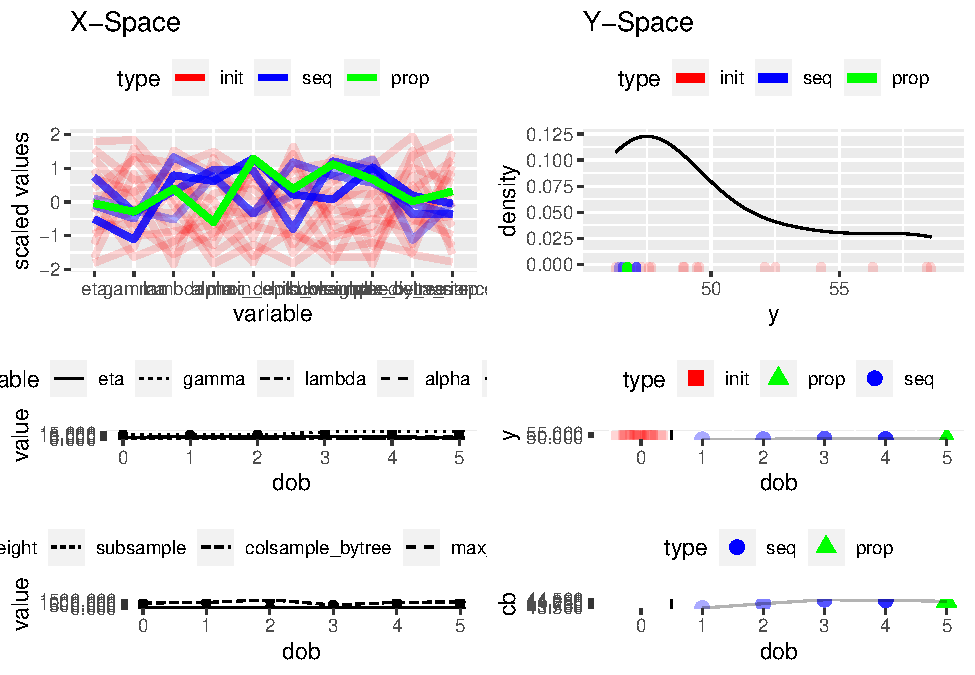
\includegraphics{Artificial-Stupidity_files/figure-latex/unnamed-chunk-29-1.pdf}

\begin{Shaded}
\begin{Highlighting}[]
\NormalTok{best.params }\OtherTok{\textless{}{-}}\NormalTok{ runs}\SpecialCharTok{$}\NormalTok{run}\SpecialCharTok{$}\NormalTok{x}

\CommentTok{\# run the model with the best hyperparamerter set}
\FunctionTok{set.seed}\NormalTok{(seed)}
\NormalTok{optimal.cv }\OtherTok{\textless{}{-}} \FunctionTok{xgb.cv}\NormalTok{(}
  \AttributeTok{params =}\NormalTok{ best.params,}
  \AttributeTok{data =}\NormalTok{ BoostTrainData,}
  \AttributeTok{nround =} \DecValTok{7000}\NormalTok{,}
  \AttributeTok{nthread =}\NormalTok{ cores,}
  \AttributeTok{nfold =}  \DecValTok{10}\NormalTok{,}
  \AttributeTok{prediction =} \ConstantTok{FALSE}\NormalTok{,}
  \AttributeTok{showsd =} \ConstantTok{TRUE}\NormalTok{,}
  \AttributeTok{early\_stopping\_rounds =} \DecValTok{5}\NormalTok{,}
  \AttributeTok{verbose =} \DecValTok{1}\NormalTok{,}
  \AttributeTok{print\_every\_n =} \DecValTok{100}\NormalTok{, }
  \AttributeTok{objective =} \StringTok{\textquotesingle{}reg:tweedie\textquotesingle{}}\NormalTok{,}
  \AttributeTok{eval\_metric =} \StringTok{\textquotesingle{}rmse\textquotesingle{}}
\NormalTok{)}
\end{Highlighting}
\end{Shaded}

\begin{verbatim}
## [1]  train-rmse:175.773471+0.346310  test-rmse:175.745911+3.113901 
## Multiple eval metrics are present. Will use test_rmse for early stopping.
## Will train until test_rmse hasn't improved in 5 rounds.
## 
## Stopping. Best iteration:
## [56] train-rmse:32.259313+0.141180   test-rmse:46.278074+1.005731
\end{verbatim}

\begin{Shaded}
\begin{Highlighting}[]
\CommentTok{\# make the final model}
\FunctionTok{set.seed}\NormalTok{(seed)}
\NormalTok{model }\OtherTok{\textless{}{-}}
  \FunctionTok{xgboost}\NormalTok{(}
    \AttributeTok{params =}\NormalTok{ best.params,}
    \AttributeTok{data =}\NormalTok{ BoostTrainData,}
    \AttributeTok{nrounds =}\NormalTok{ optimal.cv}\SpecialCharTok{$}\NormalTok{best\_ntreelimit}
\NormalTok{  )}
\end{Highlighting}
\end{Shaded}

\begin{verbatim}
## [14:58:10] WARNING: amalgamation/../src/learner.cc:573: 
## Parameters: { "tweedie_variance_power" } might not be used.
## 
##   This may not be accurate due to some parameters are only used in language bindings but
##   passed down to XGBoost core.  Or some parameters are not used but slip through this
##   verification. Please open an issue if you find above cases.
## 
## 
## [1]  train-rmse:174.459915 
## [2]  train-rmse:172.944839 
## [3]  train-rmse:171.440125 
## [4]  train-rmse:169.944763 
## [5]  train-rmse:168.458359 
## [6]  train-rmse:166.982651 
## [7]  train-rmse:165.516586 
## [8]  train-rmse:164.061493 
## [9]  train-rmse:162.617035 
## [10] train-rmse:161.183136 
## [11] train-rmse:159.762146 
## [12] train-rmse:158.352356 
## [13] train-rmse:156.954605 
## [14] train-rmse:155.568573 
## [15] train-rmse:154.196167 
## [16] train-rmse:152.836365 
## [17] train-rmse:151.489166 
## [18] train-rmse:150.157211 
## [19] train-rmse:148.838776 
## [20] train-rmse:147.534973 
## [21] train-rmse:146.245453 
## [22] train-rmse:144.971771 
## [23] train-rmse:143.713165 
## [24] train-rmse:142.472046 
## [25] train-rmse:141.246262 
## [26] train-rmse:140.038727 
## [27] train-rmse:138.848267 
## [28] train-rmse:137.674957 
## [29] train-rmse:136.519287 
## [30] train-rmse:135.382843 
## [31] train-rmse:134.264954 
## [32] train-rmse:133.165985 
## [33] train-rmse:132.071365 
## [34] train-rmse:130.995819 
## [35] train-rmse:129.941315 
## [36] train-rmse:128.905777 
## [37] train-rmse:127.890434 
## [38] train-rmse:126.847328 
## [39] train-rmse:125.852692 
## [40] train-rmse:124.828369 
## [41] train-rmse:123.824829 
## [42] train-rmse:122.831459 
## [43] train-rmse:121.857124 
## [44] train-rmse:120.898582 
## [45] train-rmse:119.981117 
## [46] train-rmse:119.042732 
## [47] train-rmse:118.116806 
## [48] train-rmse:117.204475 
## [49] train-rmse:116.309090 
## [50] train-rmse:115.428940 
## [51] train-rmse:114.565460 
## [52] train-rmse:113.715279 
## [53] train-rmse:112.894249 
## [54] train-rmse:112.063568 
## [55] train-rmse:111.249603 
## [56] train-rmse:110.448837
\end{verbatim}

\begin{Shaded}
\begin{Highlighting}[]
\CommentTok{\# take a peek}
\FunctionTok{summary}\NormalTok{(model)}
\end{Highlighting}
\end{Shaded}

\begin{verbatim}
##                Length Class              Mode       
## handle             1  xgb.Booster.handle externalptr
## raw            56424  -none-             raw        
## niter              1  -none-             numeric    
## evaluation_log     2  data.table         list       
## call              13  -none-             call       
## params            11  -none-             list       
## callbacks          2  -none-             list       
## feature_names     34  -none-             character  
## nfeatures          1  -none-             numeric
\end{verbatim}

\hypertarget{write-submission}{%
\paragraph{Write submission}\label{write-submission}}

\begin{Shaded}
\begin{Highlighting}[]
\CommentTok{\# predict }
\NormalTok{pred }\OtherTok{\textless{}{-}}
  \FunctionTok{predict}\NormalTok{(model, }\FunctionTok{model.matrix}\NormalTok{(price}\SpecialCharTok{\textasciitilde{}}\NormalTok{., testData }\SpecialCharTok{\%\textgreater{}\%} \FunctionTok{mutate}\NormalTok{(}\AttributeTok{price =} \SpecialCharTok{{-}}\DecValTok{1}\NormalTok{)) }\SpecialCharTok{\%\textgreater{}\%} \FunctionTok{xgb.DMatrix}\NormalTok{())}

\CommentTok{\# make submission csv}
\CommentTok{\# writeSubmit(pred)}
\end{Highlighting}
\end{Shaded}

\hypertarget{ann}{%
\subsubsection{ANN}\label{ann}}

This is truly an artificial stupidity. (Such a shame)

\hypertarget{build-net}{%
\paragraph{Build Net}\label{build-net}}

\begin{Shaded}
\begin{Highlighting}[]
\NormalTok{NetTrainX }\OtherTok{\textless{}{-}}\NormalTok{ trainData }\SpecialCharTok{\%\textgreater{}\%} \FunctionTok{select}\NormalTok{(}\SpecialCharTok{{-}}\NormalTok{price) }\SpecialCharTok{\%\textgreater{}\%} \FunctionTok{as.matrix}\NormalTok{() }
\NormalTok{NetTrainY }\OtherTok{\textless{}{-}}\NormalTok{ trainData }\SpecialCharTok{\%\textgreater{}\%} \FunctionTok{select}\NormalTok{(price) }\SpecialCharTok{\%\textgreater{}\%} \FunctionTok{as.matrix}\NormalTok{()}

\NormalTok{inputSize }\OtherTok{\textless{}{-}} \FunctionTok{dim}\NormalTok{(NetTrainX)[}\DecValTok{2}\NormalTok{] }
\NormalTok{offsetSize }\OtherTok{\textless{}{-}} \FloatTok{0.45}
\NormalTok{dropout }\OtherTok{\textless{}{-}} \FloatTok{0.5}
\NormalTok{activate }\OtherTok{\textless{}{-}} \StringTok{"relu"}

\NormalTok{scaleSize }\OtherTok{\textless{}{-}}\NormalTok{ inputSize }\SpecialCharTok{*}\NormalTok{ offsetSize}

\NormalTok{model }\OtherTok{\textless{}{-}} \FunctionTok{keras\_model\_sequential}\NormalTok{() }\SpecialCharTok{\%\textgreater{}\%}
  \FunctionTok{layer\_dense}\NormalTok{(}\AttributeTok{units =}\NormalTok{ scaleSize}\SpecialCharTok{*}\DecValTok{2}\NormalTok{, }\AttributeTok{activation =}\NormalTok{ activate, }\AttributeTok{input\_shape =} \FunctionTok{dim}\NormalTok{(NetTrainX)[}\DecValTok{2}\NormalTok{]) }\SpecialCharTok{\%\textgreater{}\%}
  \FunctionTok{layer\_dropout}\NormalTok{(}\AttributeTok{rate =}\NormalTok{ dropout) }\SpecialCharTok{\%\textgreater{}\%}
  \FunctionTok{layer\_dense}\NormalTok{(}\AttributeTok{units =}\NormalTok{ scaleSize}\SpecialCharTok{*}\DecValTok{4}\NormalTok{, }\AttributeTok{activation =}\NormalTok{ activate) }\SpecialCharTok{\%\textgreater{}\%}
  \FunctionTok{layer\_dropout}\NormalTok{(}\AttributeTok{rate =}\NormalTok{ dropout) }\SpecialCharTok{\%\textgreater{}\%}
  \FunctionTok{layer\_dense}\NormalTok{(}\AttributeTok{units =}\NormalTok{ scaleSize}\SpecialCharTok{*}\DecValTok{8}\NormalTok{, }\AttributeTok{activation =}\NormalTok{ activate) }\SpecialCharTok{\%\textgreater{}\%}
  \FunctionTok{layer\_dropout}\NormalTok{(}\AttributeTok{rate =}\NormalTok{ dropout) }\SpecialCharTok{\%\textgreater{}\%}
  \FunctionTok{layer\_dense}\NormalTok{(}\AttributeTok{units =}\NormalTok{ scaleSize}\SpecialCharTok{*}\DecValTok{4}\NormalTok{, }\AttributeTok{activation =}\NormalTok{ activate) }\SpecialCharTok{\%\textgreater{}\%}
  \FunctionTok{layer\_dropout}\NormalTok{(}\AttributeTok{rate =}\NormalTok{ dropout) }\SpecialCharTok{\%\textgreater{}\%}
  \FunctionTok{layer\_dense}\NormalTok{(}\AttributeTok{units =}\NormalTok{ scaleSize}\SpecialCharTok{*}\DecValTok{2}\NormalTok{, }\AttributeTok{activation =}\NormalTok{ activate) }\SpecialCharTok{\%\textgreater{}\%}
  \FunctionTok{layer\_dropout}\NormalTok{(}\AttributeTok{rate =}\NormalTok{ dropout) }\SpecialCharTok{\%\textgreater{}\%}
  \FunctionTok{layer\_dense}\NormalTok{(}\AttributeTok{units =}\NormalTok{ scaleSize}\SpecialCharTok{*}\FloatTok{0.5}\NormalTok{, }\AttributeTok{activation =}\NormalTok{ activate) }\SpecialCharTok{\%\textgreater{}\%}
  \FunctionTok{layer\_dense}\NormalTok{(}\AttributeTok{units =}\NormalTok{ scaleSize}\SpecialCharTok{*}\FloatTok{0.25}\NormalTok{, }\AttributeTok{activation =}\NormalTok{ activate) }\SpecialCharTok{\%\textgreater{}\%}
  \FunctionTok{layer\_dense}\NormalTok{(}\AttributeTok{units =} \DecValTok{1}\NormalTok{, }\AttributeTok{activation =}\NormalTok{ activate)}

\NormalTok{model }\SpecialCharTok{\%\textgreater{}\%} \FunctionTok{compile}\NormalTok{(}
   \AttributeTok{loss =} \StringTok{"mse"}\NormalTok{,}
   \AttributeTok{optimizer =}  \StringTok{"nadam"}\NormalTok{, }
   \AttributeTok{metrics =} \FunctionTok{c}\NormalTok{(}\StringTok{"mape"}\NormalTok{,}\StringTok{"mse"}\NormalTok{)}
\NormalTok{ )}
 
\NormalTok{model }\SpecialCharTok{\%\textgreater{}\%} \FunctionTok{summary}\NormalTok{()}
\end{Highlighting}
\end{Shaded}

\begin{verbatim}
## Model: "sequential"
## ________________________________________________________________________________
## Layer (type)                        Output Shape                    Param #     
## ================================================================================
## dense_7 (Dense)                     (None, 29)                      986         
## ________________________________________________________________________________
## dropout_4 (Dropout)                 (None, 29)                      0           
## ________________________________________________________________________________
## dense_6 (Dense)                     (None, 59)                      1770        
## ________________________________________________________________________________
## dropout_3 (Dropout)                 (None, 59)                      0           
## ________________________________________________________________________________
## dense_5 (Dense)                     (None, 118)                     7080        
## ________________________________________________________________________________
## dropout_2 (Dropout)                 (None, 118)                     0           
## ________________________________________________________________________________
## dense_4 (Dense)                     (None, 59)                      7021        
## ________________________________________________________________________________
## dropout_1 (Dropout)                 (None, 59)                      0           
## ________________________________________________________________________________
## dense_3 (Dense)                     (None, 29)                      1740        
## ________________________________________________________________________________
## dropout (Dropout)                   (None, 29)                      0           
## ________________________________________________________________________________
## dense_2 (Dense)                     (None, 7)                       210         
## ________________________________________________________________________________
## dense_1 (Dense)                     (None, 3)                       24          
## ________________________________________________________________________________
## dense (Dense)                       (None, 1)                       4           
## ================================================================================
## Total params: 18,835
## Trainable params: 18,835
## Non-trainable params: 0
## ________________________________________________________________________________
\end{verbatim}

\hypertarget{train-net}{%
\paragraph{Train Net}\label{train-net}}

\begin{Shaded}
\begin{Highlighting}[]
\FunctionTok{set.seed}\NormalTok{(seed)}
\NormalTok{model }\SpecialCharTok{\%\textgreater{}\%} \FunctionTok{fit}\NormalTok{(}
\NormalTok{  NetTrainX,}
\NormalTok{  NetTrainY,}
  \AttributeTok{epochs =} \DecValTok{20}\NormalTok{, }\CommentTok{\# change to make it think longer}
  \AttributeTok{batch\_size =} \DecValTok{128}\NormalTok{,}
  \AttributeTok{validation\_split =} \FloatTok{0.2}\NormalTok{,}
  \AttributeTok{verbose =} \DecValTok{2}
\NormalTok{)}

\NormalTok{scores }\OtherTok{\textless{}{-}}\NormalTok{ model }\SpecialCharTok{\%\textgreater{}\%} \FunctionTok{evaluate}\NormalTok{(NetTrainX, NetTrainY, }\AttributeTok{verbose =} \DecValTok{0}\NormalTok{)}
\FunctionTok{print}\NormalTok{(scores)}
\end{Highlighting}
\end{Shaded}

\begin{verbatim}
##       loss       mape        mse 
##   19374.35 7679282.50   19374.35
\end{verbatim}

\hypertarget{write-submission-1}{%
\paragraph{Write submission}\label{write-submission-1}}

\begin{Shaded}
\begin{Highlighting}[]
\FunctionTok{summary}\NormalTok{(model)}
\end{Highlighting}
\end{Shaded}

\begin{verbatim}
## Model: "sequential"
## ________________________________________________________________________________
## Layer (type)                        Output Shape                    Param #     
## ================================================================================
## dense_7 (Dense)                     (None, 29)                      986         
## ________________________________________________________________________________
## dropout_4 (Dropout)                 (None, 29)                      0           
## ________________________________________________________________________________
## dense_6 (Dense)                     (None, 59)                      1770        
## ________________________________________________________________________________
## dropout_3 (Dropout)                 (None, 59)                      0           
## ________________________________________________________________________________
## dense_5 (Dense)                     (None, 118)                     7080        
## ________________________________________________________________________________
## dropout_2 (Dropout)                 (None, 118)                     0           
## ________________________________________________________________________________
## dense_4 (Dense)                     (None, 59)                      7021        
## ________________________________________________________________________________
## dropout_1 (Dropout)                 (None, 59)                      0           
## ________________________________________________________________________________
## dense_3 (Dense)                     (None, 29)                      1740        
## ________________________________________________________________________________
## dropout (Dropout)                   (None, 29)                      0           
## ________________________________________________________________________________
## dense_2 (Dense)                     (None, 7)                       210         
## ________________________________________________________________________________
## dense_1 (Dense)                     (None, 3)                       24          
## ________________________________________________________________________________
## dense (Dense)                       (None, 1)                       4           
## ================================================================================
## Total params: 18,835
## Trainable params: 18,835
## Non-trainable params: 0
## ________________________________________________________________________________
\end{verbatim}

\begin{Shaded}
\begin{Highlighting}[]
\NormalTok{pred }\OtherTok{\textless{}{-}} \FunctionTok{predict}\NormalTok{(model, testData }\SpecialCharTok{\%\textgreater{}\%} \FunctionTok{as.matrix}\NormalTok{())}

\CommentTok{\# writeSubmit(pred)}
\end{Highlighting}
\end{Shaded}

\hypertarget{conclusion}{%
\subsubsection{Conclusion}\label{conclusion}}

In conclusion, there are still so much room for improvement, like
outlier handling, better NA value handling, or better clustering method.
If time is permitted, it might be better to manually implement the
essemble learning process for xgboost and mixing it with random forest
(just a thought, might need years to get it done). Other than that, the
current model (the one that produces best RMSE on kaggle) takes too long
to run (about 3 days) and most of the time are wasted on feature
selection, finding the most cluster number, and tuning XGBoost.

\end{document}
